\documentclass[twocolumn,jgrga]{AGUTeX}
\usepackage{mathptmx}
\usepackage{amssymb,amsmath}

%\usepackage{lineno}
%\linenumbers*[1]

\usepackage[pdftex]{graphicx}
\setkeys{Gin}{draft=false}

% Document metadata stuff
\authorrunninghead{STYRON AND HETLAND}
\titlerunninghead{WENCHUAN TOPOGRAPHIC STRESS}
\authoraddr{Corresponding author: Richard H. Styron, Department of Earth and
Environmental Sciences, University of Michigan, 2534 CC Little Bldg.,
1100 N. University Ave., Ann Arbor, MI 48104, USA
(richard.h.styron@gmail.com)}

\begin{document}
\title{The weight of the mountains: Constraints on tectonic stress, friction,
       and fluid pressure in the 2008 Wenchuan earthquake from estimates of 
       topographic loading}

\authors{Richard H. Styron \altaffilmark{1} and Eric A. Hetland \altaffilmark{1}}

\altaffiltext{1}{Department of Earth and Environmental Sciences, University of Michigan,
Ann Arbor, Michigan, USA.}

% document
\begin{abstract}
Though it is widely recognized that large mountain ranges produce significant
stresses in the Earth's crust, these stresses are not commonly quantified.
Nonetheless, near large mountains topography may affect fault activity by
changing the stress balance on the faults. In this work, we calculate the
stress field from topography in the Longmen Shan (Sichuan, China) and resolve
those stresses on several models of the faults that ruptured in the 2008
M$_\mathrm{w}$ 7.9 Wenchuan earthquake. We find that the topography results in
shear stresses up to 20 MPa and normal stresses up to 80 MPa on the faults,
with significant variability across the faults. Topographic stresses generally
load the fault in a normal and left-lateral shear sense, opposite to the
inferred coseismic slip sense, and thus inhibit the coseismic slip. We estimate
the accumulated tectonic stress needed to overcome topographic and lithostatic
stresses so that the direction of maximum shear on the faults is roughly
collinear with the inferred coseismic slip. We further estimate the static
friction and pore fluid pressure assuming that the fault was at Mohr-Coulomb
failure at the time of the Wenchuan earthquake. We use a Bayesian inversion
strategy, yielding posterior probability distributions for the estimated
parameters. We find most likely estimates of maximum tectonic compressive
stress near 0.6 $\rho g z$ and oriented \textasciitilde{}E-W, and minimum
tectonic stress near 0.2 $\rho g z$. Static friction on the fault is near 0.2,
and pore fluid pressure is between 0 and 0.4 of the total lithostatic pressure.
\end{abstract}


\begin{article} \section{Introduction}\label{introduction}

\begin{quote} ``And He has set up on the earth mountains standing firm, lest it
    should shake with you'' -- \emph{The Holy Qur'an}, 15:16 \end{quote}

Stress is of fundamental importance to many processes in the earth. Both the
isotropic and deviatioric components of stress exert control on the deformation
state of the earth at any point in the brittle regime. However, unlike other
fundamental quantities such as temperature, stress is typically difficult to
measure \emph{in situ}, without drilling-based techniques. Therefore, stress is
often treated in a semi-quantitative manner, with an emphasis on directions and
relative magnitudes of the principal stresses, either locally or regionally
\citep[e.g.,][]{angelier1994}. These estimates of stress are commonly derived
from strain, for example from studies of earthquake focal mechanisms
\citep[e.g.,][]{michael1987} or of fault slip data \citep[e.g.,][]{reches1987,
medinaluna2013}.

In areas of substantial relief, high terrain and steep slopes generate large
stresses in the crust beneath and adjacent to the high topography
\citep{jeffreys1924, coblentz1996}. Because of the irregularity of topography
in mountainous regions, the stresses produced by topography are also
heterogeneous, and may play a prominent role in local or regional deformation,
particularly if the region is tectonically active.  For example, shear and
normal stresses on a fault from topographic loading may push a particular fault
closer to or (as suggested by the Qur'an) farther from failure, or reorient the
net shear stress direction on a fault. These effects may affect the
localization or deformational style in a region. Furthermore, heterogeneous
topographic stresses on a particular fault may affect the way earthquake
ruptures propagate across the fault plane. Despite this, the degree to which
topographic stresses affect faulting has received little direct study.

In this work, we investigate the effects of topographic stresses on the faults
that ruptured in the 2008 \emph{M}7.9 Wenchuan, China earthquake.  This
earthquake is an ideal candidate for this study because it occurred at the base
of the Longmen Shan, one of the largest and steepest escarpments on Earth
(Figure~\ref{fig:lms_map}), and has a well-studied coseismic slip distribution
characterized by significant along-strike variations in coseismic slip.
Additionally, because the earthquake occurred after \textasciitilde{}2000 years
of seismic quiescence, postseismic stresses in the lithosphere are likely to be
negligible, suggesting that the stress state on the faults at the time of
rupture can be approximated as the sum of topographic, lithostatic, and
accumulated tectonic stresses. We then use the Mohr-Coulomb failure criterion
to bracket the tectonic stress field, pore fluid pressure, and static friction
of the fault.

\subsection{Previous work on topographic
stresses}\label{previous-work-on-topographic-stresses}

Aspects of topographic stresses and their relevance to tectonics have been
studied for some time. \citet{jeffreys1924} noted that the presence of high
mountains is evidence that the Earth's crust can support significant
heterogeneous differential stresses over long time periods.
\citet{dalmayrac1981} and \citet{molnar1988} discussed how extensional
deformation in the high parts of orogens that is temporally coincident with
contractional deformation at the low-elevation margins of the orogen may be
explained by a spatially invariant, depth-integrated horizontal compressive
stress with spatially varying vertical stresses caused by topography.
\citet{richardson1994} exploited this relationship in the central Andes to
estimate horizontal tectonic stresses through finite element modeling, and more
recently \citet{copley2009} performed similar work in Albania.
\citet{bollinger2004} showed how increased normal stress on the Main Himalayan
thrust due to loading of the high Himalayan massifs locally suppressed
microseismicity and increased fault locking. Meade and Conrad \citet{meade2008}
demonstrated that the increased weight of the uplifting Andes influenced the
Nazca-South America convergence rate.

Additionally, topographic stresses play a role in common models of orogenic
dynamics. For example, topographic loading is central to thin viscous sheet
models of lithospheric deformation \citep[e.g.,][]{birdpiper80, flesch2010gpe}.
Critical taper models for thrust or extensional wedges
\citep[e.g.,][]{dahlen1990, xiao1991} incorporate both variation in vertical
stress due to changing elevation as well as a shear stress contributed by the
slope of the wedge surface. Critical taper models also incorporate the idea
that in a growing wedge, progressively increasing topographic stresses may
eventually prevent continued slip on a given fault plane, and strain will
instead be transferred to the toe of the thrust wedge where the stress state is
more favorable. Of particular relevance to our work are `fixed boundary' models
of gravitational collapse and spreading \citep{rey2001}, where an excess of
gravitational potential energy associated with the high topography and
thickened crust of eastern Tibet causes a transfer of rock to the foreland
through horizontal contraction at the rangefront \citep[e.g.,][] {dewey1988,
liuyang2003, copleymckenzie2007}. This process may be aided by a weak
(sub)horizontal structure at depth (such as a shear zone or weak crustal
channel) that is capable of transferring the vertical and radial stresses from
topography throughout an orogen to its margins, leading to contraction there
\citep[e.g.,][]{clark2005, burchfiel2008, fleschbendick2012}.

The contributions of variable topography to the full stress field in the
elastic upper crust has been studied on smaller spatial scales.
\citet{mctiguemei1981} and \citet{savageswolfs1986} investigated the stress
components from long, symmetric ridges and showed how horizontal tension is
induced under ridge crests and horizontal compression is induced under valleys,
mostly due to shear stresses generated by slopes. Work in this vein was
continued by \citet{millerdunne1996} and \citet{martel2006}, who have focused
on shallow rock fracturing resulting from topographic stresses.
\citet{liuzoback1992} investigated whether the topographic stresses generated
by the mountains around Cajon Pass (California, USA) contributed to the
observed left-lateral shear stress on a shallow portion of the right-lateral
San Andreas fault. In their study, they developed methods for calculating the
three dimensional elastic stress tensor field arbitrary topography, whereas
previous solutions were limited to two dimensions and required topography to be
mathematically-defined (e.g., sinusoidal).

\citet{luttrell2011} inferred the coseismic shear stress changes during the
2010 \emph{Mw}8.8 Maule, Chile earthquake, and using the topographic stresses
due to the overlying fore arc, constrained the the stresses that led to this
earthquake. In their study, they calculated topographic stresses following a
similar procedure as \citet{liuzoback1992} (which we describe below), although
they only considered the component of the topographic load that can be
described by convolving a Boussinesq solution with the topography.
\citet{luttrell2011} also considered the contribution to stresses due to
buoyancy.

\subsection{The 2008 Wenchuan, China
earthquake}\label{the-2008-wenchuan-china-earthquake}

The 2008 \emph{M}7.9 Wenchuan, China earthquake is one of the most devastating
earthquakes in recent history (for an in-depth review and discussion of the
earthquake, see \citet{zhang2010}).  Surface rupture occurred along a 240 km
segment of the Beichuan fault and a parallel 72 km segment of the Pengguan
fault \citep{xu2009} (Figure~\ref{fig:lms_map}). These faults lie at the base
of the central and northeastern Longmen Shan, a mountain range that forms the
eastern margin of the Tibetan plateau. Total relief across the central Longmen
Shan is around 4 km, though relief subsides somewhat to the northeast.  The
central and southwestern Longmen Shan is the steepest margin of the Tibetan
plateau \citep{clarkroyden2000} and one of the highest and steepest escarpments
on earth. This is most apparent in the southwestern portion of the earthquake
rupture, where elevations \textgreater{} 4000 m over the Pengguan massif (a
Precambrian crystalline massif in the hanging wall of the Beichuan thrust) drop
to \textasciitilde{}1200 m in as little as 6 km map distance.

\begin{figure*}[ht!] \includegraphics[width=40pc]{../figures/lms_map.pdf}
    \caption{Map of eastern Tibet and the Sichuan basin, showing active
        structures from \citet{styron2010}. Faults that ruptured in the 2008
        Wenchuan earthquake are shown in pink. GPS velocities are relative to
        the mean velocity of sites within Sichuan basin, with 1$\sigma$
        uncertainty, from the dataset of Liang et al.  \citet{liang2013}.
        Beachball is from the Global CMT focal mechanism solution for the 2008
    Wenchuan earthquake. BF = Beichuan fault. PF = Pengguan fault. P = Pengguan
massif. Grey box shows the extent of Figures 3 and 9.} \label{fig:lms_map}
\end{figure*}

Surface ruptures during the Wenchuan earthquake are highly variable and show
vertical (reverse-sense) displacements up to 9 m and horizontal (right-lateral
sense) displacements up to 5 m \citep{lin2009, liu2009, xu2009}. In general,
vertical displacements are higher in the southwestern to central portions of
the Beichuan rupture and decrease in the northeast, whereas horizontal offsets
are higher in the central to northeast, though considerable variation exists.
Coseismic slip models constrained by seismic and geodetic data reveal a
complicated pattern of coseismic slip in the Wenchaun earthquake, with several
high-slip patches that dominate the seismic moment release and significant
variation coseismic slip rake along strike \citep[e.g.,][]{nakamura2010,
shen2009, tong2010, feng2010, zhang2011, qi2011, fielding2013}.  The variation
in rake is such that the southwest portions of the fault slipped largely in a
reverse sense, while the northeast portions sliped largely in a right-lateral
sense. This change in rake is associated with a change in inferred fault dip.
Sections of faults that ruptured in the Wenchuan earthquake (which we simply
refer to as the ``Wenchuan earthquake faults'') with shallow to moderate dips
largerly ruptured as thrust, and sections with steeper dips largely ruptured as
strike-slip.  \citet{medinaluna2013} concluded that this relationship is
consistent with a uniform orientation of principal stresses, where the
variation of the dip of the fault leads to a change in the direction of maximum
fault shear stress, which they assumed to be parallel to the coseismic slip
rake.

\subsection{This study}\label{this-study}

We seek to quantify the topographic stress field in the Longmen Shan region,
and on the Wenchuan earthquake faults themselves. Specifically, we evaluate the
extent to which topographic stresses promote or inhibit slip in the 2008
Wenchuan earthquake. If topographically induced shear stresses on the fault are
in roughly in the same direction as the coseismic slip, then topographic
loading general promotes coseismic slip (Figure \ref{fig:topo_fault_scenarios}
a). On the other hand, if the topographic shear stresses are roughly in the
opposite direction of coseismic slip, then topographic loading inhibits
coseismic slip (Figure \ref{fig:topo_fault_scenarios} b). If topographic
loading resisted slip across the Beichuan faults, then tectonic stresses would
need to counteract the topographic fault stresses for the coseismic slip to
result. On a smaller scale, the heterogeneity of coseismic slip in the
earthquake may be influenced by shorter wavelength variations in topography and
topographic stresses.

\begin{figure*}[t!] \centering
    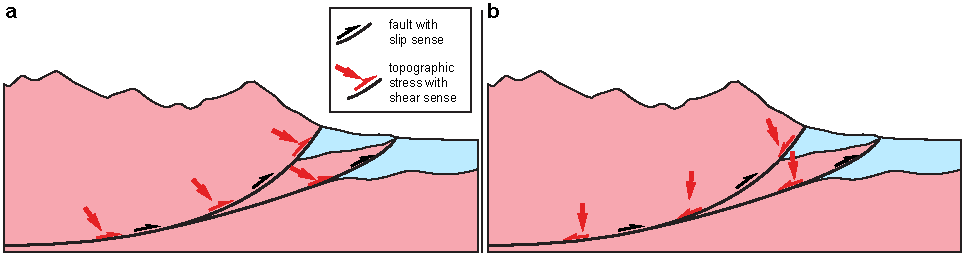
\includegraphics[width=40pc]{../figures/topo_stress_possibilities.pdf}
    \caption{Scenarios for topographic effects on rangefront thrust faulting.
        (a) Topographic stresses promote thrust faulting. (b) Topographic
        stresses inhibit thrust faulting.} \label{fig:topo_fault_scenarios}
    \end{figure*}

Topographic stresses are only one component of the total stress field in the
crust \citep{molnar1988}. Coseismic slip in the Wenchaun earthquake is due to
the total accumulated stress on the faults, which also includes components from
lithostatic and tectonic stresses. (In the present study, we do not consider
stresses due to flexure \citep[e.g.,][] {luttrell2007} or buoyancy
\citep[e.g.,][]{luttrell2011}.) By quantifying both the topographic and
lithostatic stresses, we can use coseismic slip models to solve for the
tectonic stress assuming that (1) the total shear stress on the fault is in the
direction of coseismic slip \citep[e.g.,] []{angelier1994} and (2) the fault is
at Mohr-Coulomb failure everywhere that it slipped. If topographic stresses are
significant and produce shear in the direction of fault slip, then for given
values of static friction and pore fluid pressure, we can calculate the amount
of tectonic stress that can be added to the ambient stress field before the
faults should rupture; given limited acceptable ranges for friction and fluid
pressure, we are essentially able to place maximum constraints on tectonic
stress. Alternately, if topographic stresses work against coseismic slip, for
given friction and fluid pressures we can estimate the minimum magnitudes of
tectonic stresses necessary to overcome shear and frictional resistance to
slip. In a scenario with complex faulting and topography, it may be possible to
put tight bounds on minimum and maximum magnitudes and directions of tectonic
stresses. To account for the non-uniqueness of the solution, we use a Bayesian
Monte-Carlo methodology to estimate posterior probability density functions
(PDFs) of tectonic stresses, static fault friction, and pore fluid pressure.

\section{Topographic stresses on the Longmen Shan
faults}\label{topographic-stresses-on-the-longmen-shan-faults}

To quantify tectonic stresses on the Wenchuan earthquake faults, we
first calculate the topographic stress field in the upper crust
throughout eastern Tibet, then interpolate those stresses onto three
dimensional models of the faults taken from coseismic slip models.
Finally, we calculate topographic shear and normal stresses on the
faults and compare those to the coseismic slip patterns.

\subsection{Topographic stress tensor field
calculations}\label{topographic-stress-tensor-field-calculations}

We calculate the stress tensor field induced by topography throughout
eastern Tibet using methods developed by 
\citet{liuzoback1992}. They show that the topographic stress tensor
field can be determined by a convolution of topographic loading
functions with Green's functions describing the stresses in an elastic
halfspace due to a point load at the surface. In our notation, the
stress tensor field due to topography is given by

\begin{equation}
M(x, y, z) = G(x, y, z) * F(x, y) \; ,
\end{equation}

where $G(x,y,z)$ is a set of Green's functions for the six stress tensor
elements, and $F(x,y)$ is a topographic loading function, described
below. We assume compressive stresses are positive, and $x>0$ is east,
$y>$ is north, and $z>0$ is depth. \citet{liuzoback1992}
show that $M(x,y,z)$ can be decomposed into two components as

\begin{equation}
M(x,y,z) = M^B(x,y,z) + M^C(x,y,z) \; .
\end{equation}

$M^B(x,y,z)$ is the component of the stress field due to the vertical
loading of the topography, and is

\begin{equation}
M^B(x, y, z) = G^B(x,y,z) * F_v(x, y) \; ,
\label{eqn:bous}
\end{equation}

where $G^B(x,y,z)$ are the Boussinesq solutions for stresses in a
halfspace due to a vertical point load on the surface (see Appendix A1), 
$F_v(x,y) = \rho g h(x,y)$, and $h(x,y)$ is topography. 
Note that $h(x,y)<0$ since $z<0$ is
depth. $M^C(x,y,z)$ is the component of the stress field due to the
mechanical coupling of the topography to the half-space, i.e.,
describing the lateral spreading forces in the rock above the halfspace,
and is given by

\begin{equation}
M^C(x, y, z) = G_x^C(x,y,z) * F_{h, x}(x, y) + G_y^C(x,y,z) * F_{h, y}(x, y) \; ,
\end{equation}

where $G_i^C(x,y,z)$ are the Cerruti solutions for a horizontal point
source load in the $i$ direction on the halfspace surface (see Appendix
A1). The horizontal loading functions are given by

\begin{equation}
\begin{split}
F_{h, \, x}(x,y) = ( \rho g h(x,y) + M_{xx}^B(x,y,0) + T_{xx} )\, \frac{\partial h}{ \partial x} \\
\quad + (M_{xy}^{B}(x,y,0) + T_{xy}) \frac{\partial h}{ \partial y}
\end{split}
\label{eqn:f_hor_xz}
\end{equation}

and

\begin{equation}
\begin{split}
F_{h, \, yz}(x,y) = ( \rho g h(x,y) + \sigma_{yy}^B(x,y,0) + T_{yy} )\, \frac{\partial h}{ \partial y} \\
\quad + (M_{xy}^{B}(x,y,0) + T_{xy}) \frac{\partial h}{ \partial x}\; . 
\end{split}
\label{eqn:f_hor_yz}
\end{equation}

$M_{ij}^B(x,y,0)$ is the stress from the vertical (Boussinesq) load
evaluated at $z=0$, and $T_{ij}$ is the tectonic stress component, which
we neglect in the present calculations.

\subsection{Numerical implementation}\label{numerical-implementation}

Topography was taken from the CGIAR-CSI v.4 release
\citep{jarvis2008srtm} of the Shuttle Radar Topographic Mission
\citep{farr2007srtm} Digital Elevation Model (DEM) at 1 km nominal
resolution. The DEM was projected from native WGS84 geographic
coordinates to UTM zone 48N, decreasing the nominal horizontal
resolution to 851 m. We assume a Poisson halfspace, and Green's
functions for the Boussinesq and Cerruti point-source solutions were
calculated at regular points in large 2-D grid at each depth
considered, with the point-source centered in the grid (see Table
\ref{table:convo_params} for model parameters). A mask was applied to
each of the discretized Green's functions such that values outside a 
radius (i.e. the `corners' of the array) were set to zero, yielding a
circular array. The size of the
grid was chosen to be quite large to incorporate potential contributions
from the elevated topography throughout eastern Tibet. So that the
Green's functions and the topography were discretized on the same size
grid, we pad the Green's function array with zeros. Because of
singularities in the Green's functions at $z=0$, we use
$\sigma^B(x,y,z)$ with $z=851$ m, the shallowest level of our
calculations, in construction of the horizontal loading functions in
Equations \ref{eqn:f_hor_xz} and \ref{eqn:f_hor_yz}. Convolutions were
computed using a 2D fast Fourier transform. All calculations were
implemented in Python (v. 2.7.3) using IPython \citep{perez2007ipython},
NumPy (v. 1.7) \citep{oliphant2007numpy} and Pandas (v. 12)
\citep{mckinney2010}; additional statistical analysis was performed with
StatsModels \citep{seabold2010}. We created an open-source Python package
to calculate topographic stresses in a reasonably automated way, which
is available at \url{https://github.com/cossatot/halfspace}. The package
is being expanded to encompass a wide range of elastic stress and strain
solutions as time permits. All data and scripts for this particular
project are available at
\url{https://github.com/cossatot/wenchuan_topo_stress}.

\begin{table}
\centering
\begin{tabular}{l c l}
\hline
Parameter & Value & Unit \\
\hline
horizontal spacing & 851 & m \\ 
vertical spacing & 1000 & m \\ 
minimum depth & 851 & m (below sea level) \\ 
maximum depth & 35851 & m (below sea level) \\ 
density ($\rho$) & 2700 & kg m$^{-3}$ \\ 
g & 9.81 & m s$^{-2}$ \\ 
Green's function radius & 9e5 & m \\ 
Poisson ratio & 0.25 & - \\ 
\hline
\end{tabular}
\caption{Parameters for numerical calculations of topographic stresses.}
\label{table:convo_params}
\end{table}

\subsection{Topographic fault stress
calculations}\label{topographic-fault-stress-calculations}

Topographic stresses on the Wenchuan faults are calculated on point sets
representing the faults taken from coseismic slip models. We use the
coseismic slip models of \citet{shen2009},
\citet{feng2010}, \citet{qi2011}, \citet{zhang2011},
and \citet{fielding2013}, and discard
points above 851 m below sea level, as this is above the depth at which
we compute $G^C(x,y,z)$. The six stress tensor components calculated at
the regular grid points are linearly interpolated to points describing
the faults. Because the fault points are completely surrounded by the
grid nodes at which topographic stresses were calculated and those nodes
are spaced \textless{}1 km apart, the fault points cannot be more than a
few hundred meters from the nearest grid node, so a higher order
interpolation is not necessary. We then project the topographic stress
tensor to fault normal stress, $\sigma_n^M$, down-dip shear stress,
$\tau_d^M$ and strike-slip shear stress, $\tau_s^M$ at each point in
describing the fault geometry.

\section{Results of topographic stress calculations on the Wenchuan
faults}\label{results-of-topographic-stress-calculations-on-the-wenchuan-faults}

Topographic stresses on the Wenchuan faults are on the order 1--10s MPa
(Figure~\ref{fig:lms_topo_stresses_rot}, ~\ref{fig:fault_stress_3d}). 
Stresses are highest in the southwest,
beneath the Pengguan massif (the highest topography of the Longmen Shan
front), and decrease to the northeast. $M_{zz}$ is typically larger,
though not substantially, than $M_{xx}$ or $M_{yy}$. Maximum horizontal
stress is not typically aligned with either cardinal horizontal
direction, and is typically larger than $M_{zz}$ above 10 km. Maximum
$M_{zz}$ is near 80 MPa, on the southwestern Beichuan fault below the
high peaks of the Pengguan massif, except for in slip models containing
near-horizontal fault segments in the mid-crust, where $M_{zz}$ reaches
100 MPa. Vertical shear stresses ($M_{xz}$ and $M_{yz}$) are on the
order of 1 MPa, and horizontal shear stress ($M_{xy}$) is on the order
of 0.1 MPa.

\begin{figure}[t]
\centering
\includegraphics[width=20pc]{../figures/lms_topo_stresses_rot.pdf}
\caption{Horizontal topographic stresses in the Longmen Shan region at 5
km depth: black and red lines signify most and least compressive
horizontal stresses, respectively. Other symbols are the same as in Figure
1. Stresses shown are down-sampled from the
discretization used in the calculations by a factor of six.}
\label{fig:lms_topo_stresses_rot}
\end{figure}

Because the compressive stresses are near equal, $M$ contains a large
isotropic component and a smaller deviatoric component. Consequently, $M$
resolves on the Wenchuan faults with a large $\sigma^M_n$ (median of
about 40-60 MPa for each slip model) and much smaller $\tau^M_d$. The
median $\tau^M_d$ is about -3 to -6 MPa in each slip model, where values
less than zero indicate normal-sense shear, and $\tau^M_s$ median values
range from about -2 to 1 MPa, where values less than zero indicate
sinistral shear; fault models with positive median $\tau^M_s$ have broad
thrust flats at depth, where little slip occurred. On the steeper fault
segments (where most of the moment release occurred), topographic shear
stresses are typically normal-sinistral, as opposed to the dominant mode
of coseismic slip, which is reverse-dextral.

\begin{figure*}[htbp]
\centering
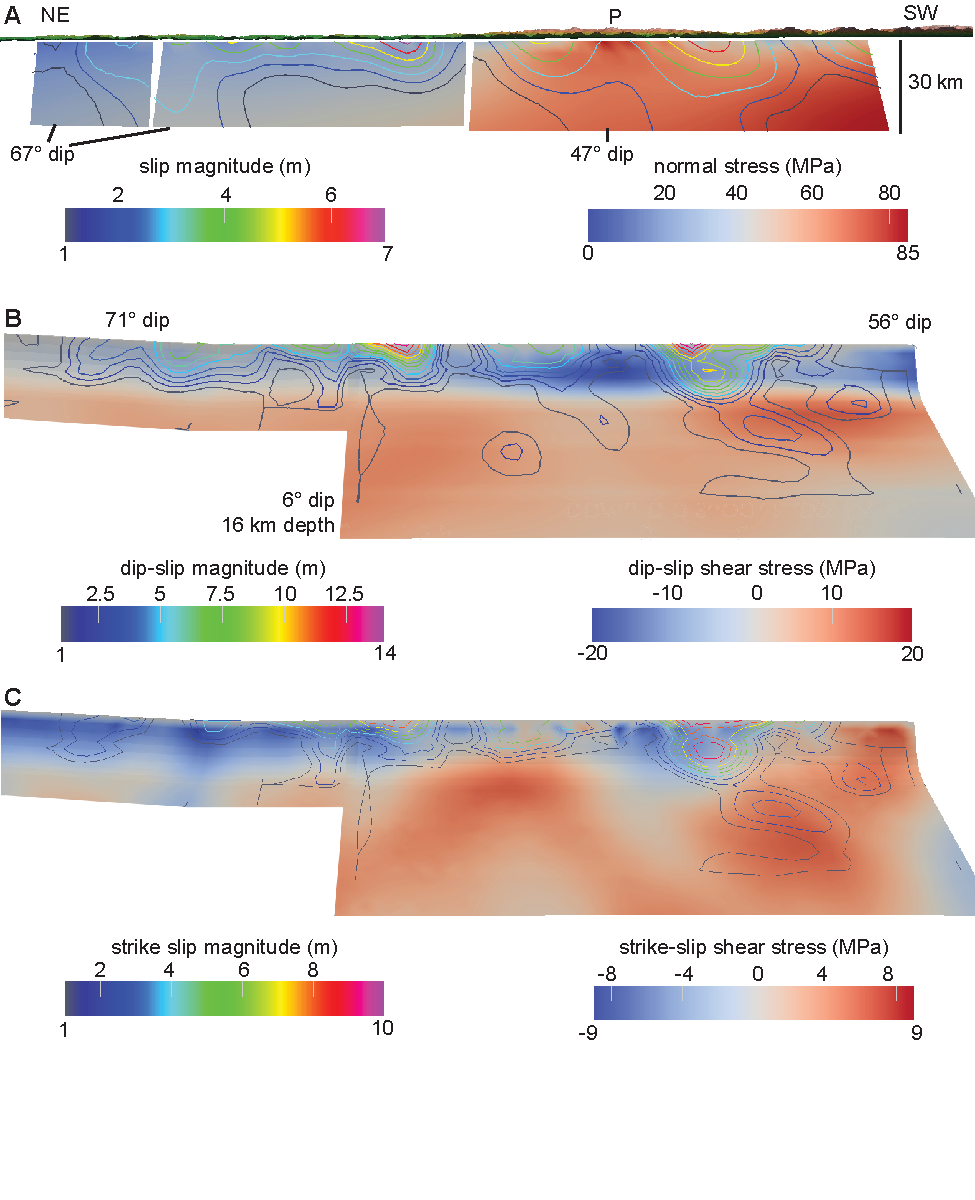
\includegraphics[width=40pc]{../figures/fault_stress_3d.pdf}
\caption{Southwest-looking views of topographic stresses and coseismic
slip on selected slip models. All models share same lateral extent, but
the perspectives for B and C are more inclined than A. (A) $\sigma_n^M$
(colors), slip magnitude (contours, 1 m interval) and hanging-wall
topography on the \citet{feng2010} model of the Beichuan
fault. Note the suppression of fault slip where normal stress is
highest, such as below the Pengguan massif (P). Fault and topography
share the same scale, with no vertical exaggeration. (B) $\tau_d^M$ (colors)
and dip slip (contours, 1 m interval) on the \citet{qi2011}
`rough' slip model. (C) $\tau_s^M$ (colors) and strike slip (contours, 1
m interval) on the \citet{qi2011} slip model.}
\label{fig:fault_stress_3d}
\end{figure*}

In contrast to the steeper fault segments, much of the shallowly-dipping
fault segments (the Pengguan fault and flats at the base of the Beichuan
fault, where present) have $\tau^M$ in the direction of coseismic slip.
$M$ is not significantly different in these
locations, but because of the low dip angle, $M_{zz}$ contributes more
significantly to $\sigma^M_n$ than to $\tau^M_d$, which is then
dominated by horizontal compression, leading to reverse-sense shear.
The stresses caused by the Pengguan massif locally resolve
as right-lateral on these segments as well. Coseismic slip on these
fault patches is much lower than on the steeper Beichuan fault, where
the majority of slip occurred and which is topographically loaded in the
opposite shear sense.

Compellingly, similar patterns exist in the spatial distributions of
$\sigma^M_n$ and coseismic slip. Most obvious is the coincidence of
locally high $\sigma^M_n$ and locally low slip magnitude on the
southwestern Beichuan fault below the culmination of the Pengguan
massif, in an area of otherwise high slip (Figure
\ref{fig:fault_stress_3d}). These correlations exist for other fault
patches, but they are not as clear (Figure
\ref{fig:feng_slip_sig_n_scatter}). This raises the possibility that
topographic loading of these faults contributes to limiting coseismic
slip once failure has occurred, and
may have implications for estimations of dynamic friction and the
completeness of stress drop during the earthquake. Preliminary analysis
of this is currently being performed, and will be described in a
forthcoming manuscript.

\begin{figure}%[htbp]
\centering
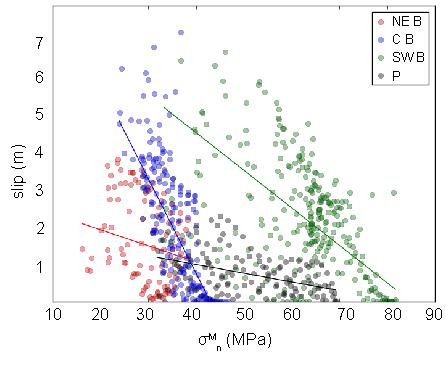
\includegraphics[width=20pc]{../figures/feng_slip_sig_n_scatter.pdf}
\caption{Coseismic slip magnitude and $\sigma^M_n$ on the four segments
of the \citet{feng2010} coseismic slip model. Trendlines are
L1 regressions and do not include points with no slip. ``NE B'' =
Northeastern Beichuan fault. ``C B'' = central Beichuan fault. ``SW B'' =
Southwestern Beichuan fault. ``P'' = Pengguan fault.}
\label{fig:feng_slip_sig_n_scatter}
\end{figure}

\section{Calculations of tectonic stress, fault friction and pore fluid
pressure}\label{calculations-of-tectonic-stress-fault-friction-and-pore-fluid-pressure}

Faults fail in earthquakes when the shear stresses on the fault overcome
the frictional stresses resisting slip on the fault \citep[e.g.,][]
{scholz2002}. We assume that the entire fault was at at the point of
failure when the Wenchuan fault initiated, and use the Mohr-Coulomb
failure criterion

\begin{equation} 
\tau = \mu ( \sigma_n - \sigma_p ) \; ,
\label{eqn:amonton_raw} 
\end{equation}

where where $\mu$ is the coefficient of static friction on the fault and
$\sigma_p$ is the pore fluid pressure \citep[e.g.,][]{sibson1985}. We
describe the pore fluid pressure using a scalar, $0 \leq \phi \leq 1$,
which is the pore fluid pressure as a fraction of total pressure, and so
the failure criterion is

\begin{equation} 
\tau = \mu (1 - \phi) \sigma_n \; 
\label{eqn:amonton} 
\end{equation}

\citep[e.g.,][]{sibson1985}. We assume that both $\mu$ and $\phi$ are
constant across the Wenchuan faults.

We estimate the tectonic stress tensor field, $\mu$, and $\phi$
consistent with published coseismic slip models of the Wenchuan
earthquake using a Bayesian estimation, resulting in posterior probability 
density functions of the model parameters. 
We first estimate posteriors of $T$ cosistent with
the coseismic slip models, and then estimate $\mu$ and $\phi$ consistent
with Mohr-Coulomb failure. The nature of Bayesian estimation allows us
to quantify both the relative likelihoods of model parameters and the
tradeoffs between them.

\subsection{Description of the stress
state}\label{description-of-the-stress-state}

We consider the complete stress tensor, $S$, at a point in the crust to
be

\begin{equation}
S = M + T + L \; ,
\end{equation}

where $M$ is described above, $T$ is the tectonic stress tensor, and $L$
is the lithostatic stress tensor. $L$ is isotropic, with diagonal
components equal to $\rho g z$. We assume that $T$ is latterally
homogeneous and only has horizontal stress components (i.e.,
$T_{xz} = T_{yz} = T_{zz} = 0$, with $T_{xx}$, $T_{yy}$ and $T_{xy}$
non-zero). We further assume that $T$ increases linearly with depth so
that the entire upper crust is near the critical failure envelope
\citep[e.g.,][]{townend2000}, are thus we parameterize the components of $T$
as scalars multiplied by lithostatic pressure, denoted as $T^\prime$

\subsection{Bayesian inversion of tectonic
stresses}\label{bayesian-inversion-of-tectonic-stresses}

We invert topographic stresses and coseismic slip models for tectonics
stresses using Bayesian methods, and making the common `Wallace-Bott'
assumption (named after \citet{wallace1951} and \citet{bott1959}) 
that slip on the fault occurs in the general direction
of the maximum resolved shear stress on the fault \citep[e.g.,][]
{mckenzie1969, angelier1994}. We estimate the tectonic stresses in
light of the topographic stresses and slip distributions through the
relation

\begin{equation} 
p(T|D) \propto p(T) \, p(D|T) \; , 
\label{eqn:bayes_rule} 
\end{equation}

where $p(T)$ is the prior PDF (or \emph{priors}) of $T$, $p(D|T)$ is the
likelihood of observing the coseismic slip distribution $D$ given the
tectonic stresses $T$, and $p(T|D)$ is the posterior PDF of $T$ given
$D$, which is the solution to the inversion \citep[e.g.,][]{mosegaard1995}.
Due to the unknown proportionality in equation (\ref{eqn:bayes_rule}),
our posterior only gives likelihood of $T$ relative to the most likely
estimate (MLE) \citep{tarantola2005}. We follow a Monte-Carlo strategy,
where samples of the prior PDF are retained as samples of the posterior
in proportion to $p(D|T)$ \citep[e.g.,][]{mosegaard1995}.

We parameterize $T$ by the magnitudes and orientation of the maximum and
minimum principal tectonic stresses. We assume priors such that the
magintudes of principal tectonic stresses are equally likely within
bounds and that all orientations are equally likely. Because the
Wenchuan event was an oblique reverse faulting earthquake, we assume
that total horizontal stresses are greater than the vertical stress,
which is satisfied if the tectonic stresses are positive. Prior samples
of maximum principal stress are taken from a uniform distribution
between $\rho g z$ and 2.5 $\rho g z$. Samples of the minimum principal
stress are from a uniform distribution between 0 and the value for
maximum stress. We describe the orientation of the tectonic stress using
the azimuth of the maximum tectonic stress, which are sampled uniformly
from 0 to 360$^{\circ}$.

We test 100,000 unique samples drawn from the prior using a seeded
pseudorandom number generator. We test the same prior samples against
each of the coseismic slip models. $S$ is then constructed for each
point discretizing the fault geometries in the coseismic slip models.
The rake of the maximum shear stress $\lambda^S$ on each point of the
fault is calculated and compared to the coseismic slip rake $\lambda^D$
at that point. A weighted mean misfit is calculated by

\begin{equation}
\bar{\lambda}^m = \sum \nolimits_{i=1}^n \frac{(\lambda^S_i - \lambda^D_i) D_i} 
{\bar{ D}} \; ,
\label{eqn:rake_misfit}
\end{equation}

where $D$ is the coseismic slip and $\bar{D}$ is the average coseismic
slip in a given coseismic slip model. Finally, the relative likelihood
of each model is computed using a Von Mises distribution as

\begin{equation}
p (D | T) = \frac{ \exp ( \kappa \cos \bar{\lambda}^m )} 
{\exp (\kappa \cos \bar{\lambda}^m_{\min})} \;,
\label{eqn:rel_likelihood}
\end{equation}

where $\kappa$ = 8.529, which is calculated so that the 68.2\%
confidence interval the Von Mises distribution is within $\pi$/9 radians
(20$^{\circ}$), the estimated 1$\sigma$ uncertainty of the coseismic
slip models based on comparisons between rakes of high-slip fault
patches (note that for a planar fault, $\tau$ at $\pi/9$ radians from
$\lambda_{max}$ is still \textgreater{}90\% of $\tau_{\mathrm{\max}}$
\citep{lisle2013}). Prior samples are retained in propotion to $p(D|T)$,
and the retained samples are then samples of the posterior.

\subsection{Analysis of friction and pore fluid
pressure}\label{analysis-of-friction-and-pore-fluid-pressure}

Once the tectonic stress distributions consistent with the coseismic
slip models have been determined, we deduce the distributions of $\mu$
and $\phi$ assuming that the stress is at the failure criterion in
equation (\ref{eqn:amonton}). We do this in three steps: First, we draw
a random $\phi$ from a uniform distribution, assuming $0 \leq \phi < 1$.
We again use a seeded pseudorandom number generator, such that each
stress model has a uniquely assigned $\phi$ that is consistent priors
accross all coseismic slip models. Second, we calculate $\tau^S$ and
$\sigma_n^S(1-\phi)$ for each point on the fault. Third, we solve
Equation \ref{eqn:amonton} for $\mu$. Finally, we filter the results so
that only models with $0 \le \mu < 1$ are retained, as values outside of
that range have not been suggested for rocks.

After this analysis has been done for all coseismic slip model, we find
the joint posterior (i.e., the posterior consistent with all of the
coseismic slip models) by taking the samples that are common to all of
the individual posteriors. We denote the joint posterior as
$p_{\mathrm{J}}(P | D)$, where $P$ is the parameter of interest.

\section{T, $\mu$, $\phi$ results}\label{t-mu-phi-results}

\subsection{Individual slip models}\label{individual-slip-models}

Results for $T^\prime$, $\mu$ and $\phi$ are quite consistent across all
coseismic slip models (Figure \ref{fig:T_scatters}). Maximum compressive
stress $T^\prime_{\mathrm{max}}$ is broadly east-west for all models,
with a mode trending at $90^{\circ}$--$105^{\circ}$.
$p(T^\prime_{\mathrm{max}}|D)$ for each slip model increases from
$T^\prime = 0$ to 0.5 or 1 before essentially leveling off, though some
slip models, particularly the \citet{qi2011} model, show a
slight decrease in relative likelihood past the initial mode at
$T^\prime =$ 0.5--1.
The low likelihood below $T^\prime \approx 0.5$ indicates that lower
tectonic stresses are unlikely to overcome fault friction and
topographic shear stresses resisting reverse-dextral slip on the
Wenchuan faults. $p(T^\prime_{\mathrm{min}} | D)$ for each slip model
has a mode close to $T^\prime_{\mathrm{min}} = 0.2 $ and decreases
abruptly at higher values, though all slip models show values for
$T^\prime_{\mathrm{min}}$ up to 2.5. $T^\prime_{\mathrm{min}}$ is
typically 0--0.4 of $T^\prime_{\mathrm{max}}$, but rarely higher.

\begin{figure*}%[htbp]
\centering
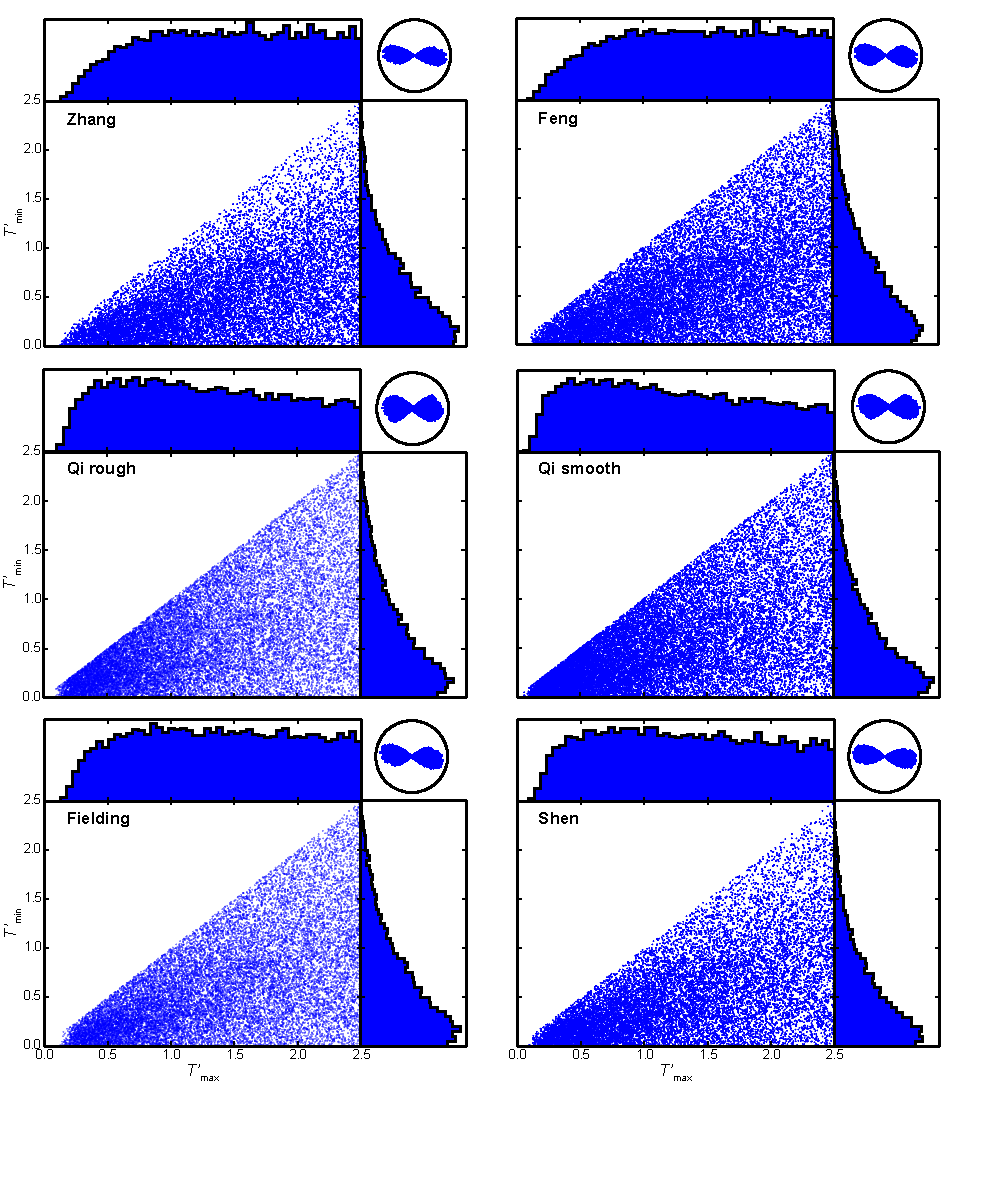
\includegraphics[width=40pc]{../figures/T_scatters.pdf}
\caption{Samples of
$p(T^\prime_{\mathrm{max}},T^\prime_{\mathrm{min}} | D)$ associated with
each of the coseismic slip models we consider, along with marginals of
$T^\prime_{\mathrm{max}}$ and $T^\prime_{\mathrm{min}}$. Inset rose
diagrams are histograms of azimuth of
$T^\prime_{max}$.}
\label{fig:T_scatters}
\end{figure*}

All slip models show $p(\phi | D)$ to be uniformly high from $\phi = 0$
to 0.4--0.6 and to decrease linearly to $p(\phi) = 0$ at $\phi = 1$
(Figure \ref{fig:mu_phi_scatters}). $p(\mu | D)$ for all slip models has
a mode at $\mu =$ 0.1--0.4 and $p(\mu)$ decreases at higher values.
$T^\prime_{\mathrm{max}}$, $\phi$ and $\mu$ are highly correlated, where
higher values of $T^\prime_{\mathrm{max}}$ are associated with higher
$\mu$ and lower $\phi$. Combinations of high $\mu$ and low $\phi$
require much higher $T^\prime_{\mathrm{max}}$ to overcome fault friction
and cause slip, and so are not represented in the posteriors. Since our
maximum $T_{\mathrm{max}}$ of $2.5 \rho g z$ is quite high
($\approx 660$ MPa at 10 km), we view high $\mu$ and low $\phi$
combinations as unrealistic for the Wenchuan faults. Similarly,
combinations of very low $\mu$ and very high $\phi$ are associated with
very low $T^\prime_{\mathrm{max}}$, and have a low probability density,
as it is unlikely that tectonic stress with very low $T^\prime_{\mathrm{max}}$
values can
overcome sinistral and normal-sense topographic shear stresses to cause
the observed coseismic slip kinematics.

\begin{figure*}[htbp]
\centering
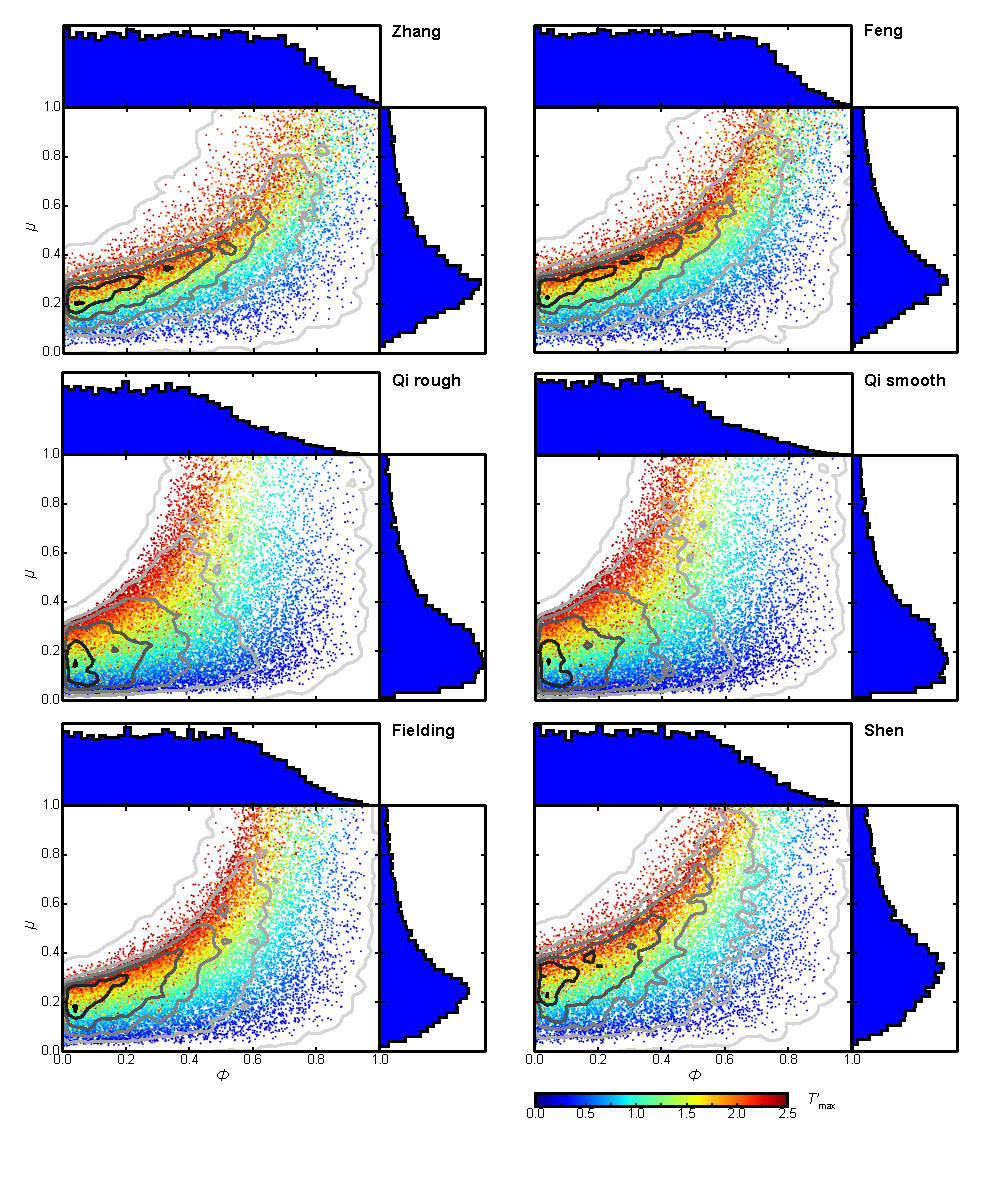
\includegraphics[width=40pc]{../figures/mu_phi_fms.pdf}
\caption{Samples of $p(\mu,\phi | D)$ for each coseismic slip model.
Colors indicate magnitude of $T^\prime_{\mathrm{max}}$. Contour lines
indicate relative density (i.e., likelihood) of posteriors (darker lines
signify higher densities).}
\label{fig:mu_phi_scatters}
\end{figure*}

\subsection{Joint posteriors}\label{joint-posteriors}

We define a joint posterior, $p_{J}(T^\prime | D)$, by the samples that 
are common to the individual posteriors estimated from each slip model.
Unsuprisingly, given the broad similarity between the posteriors from
the various slip models, $p_{J}(T^\prime_{\mathrm{max}} | D)$ is not
substantially different from any of the constituent model posteriors.
$p_{J}(T^\prime_{\mathrm{max}} | D)$ has a somewhat more well-defined
mode at $T^\prime_{\mathrm{max}} \approx 0.6$.

In our estimation of $\phi$ and $\mu$ in the posteriors associated with
each slip model, we have used the same random combinations of $T$ and
$\phi$ for each slip model, and then solved for $\mu$ so that the fault
is at a critical stress state (Equation \ref{eqn:amonton}). Because of
differences in the location and slip among the coseismic slip models,
some variability exists in $\mu$ for each prior sample. We therefore
choose $p_{\mathrm{J}}(\mu | D)$ to be the median $\mu$ of each slip
model for each sample. $p_{\mathrm{J}}(\mu | D)$ has a mostly similar
distribution as $p(\mu | D)$ for any of the slip models. However,
$p_{\mathrm{J}}(\mu | D)$ has a lower relative likelihood on the
high-$\mu$ tail compared to the constituent $p(\mu | D)$. This lower
likelihood of $\mu$ in the joint posterior is likely becuase it is the
average $\mu$ of all slip models. On the other hand, it is not similarly
sparse on the low-$\mu$ side, suggesting that low values for $\mu$ are
more robust.

\begin{figure*}[t]
\centering
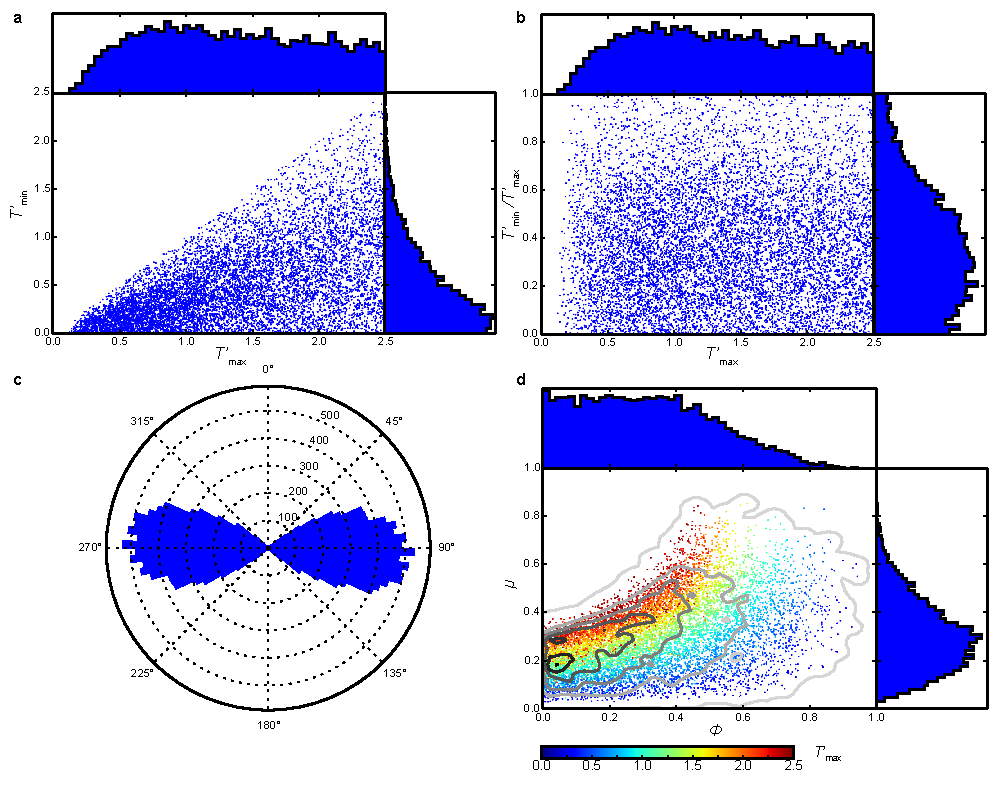
\includegraphics[width=40pc]{../figures/joint_pdfs.pdf}
\caption{(a) Samples of
$p_{\mathrm{J}}(T^\prime_{\mathrm{max}},T^\prime_{\mathrm{min}} | D)$,
along with marginals of $T^\prime_{\mathrm{max}}$ and
$T^\prime_{\mathrm{min}}$. (b) Samples of
$p_{\mathrm{J}}(T^\prime_{\mathrm{\max}}, T^\prime_{\mathrm{\min}}/T^\prime_{\mathrm{max}} | D)$,
along with marginals of $T^\prime_{\mathrm{max}}$ and
$T^\prime_{\mathrm{min}} / T^\prime_{\mathrm{max}}$. (c) Histogram of
azimuths of $T^\prime_{\mathrm{\max}}$. (d) Samples of
$p_{\mathrm{J}}(\mu, \phi | D)$, with marginals, where color of the samples
indicate magnitudes of $T^\prime_{\mathrm{\max}}$ and contour
lines indicate relative density (i.e., likelihood) of posteriors (darker
lines signify higher densities).}
\label{fig:joint_posteriors}
\end{figure*}

\section{Discussion}\label{discussion}

Few studies have performed similar quantification of static stress
fields on faults (see Section
\ref{previous-work-on-topographic-stresses} for some examples), even
though it may have important ramifications to the earthquake process.
Most studies of fault rupture dynamics
assume either a homogeneous or stochastic shear stress distribution
\citep[e.g.,][]{oglesbyday2002} and few assume any variation in normal
stress \citep[e.g.,][]{aagaard2001}, despite the importance that stress
variations likely have in earthquake dynamics \citep[e.g.,][]{day1982,
olsen1997}. Additionally, quantifying friction and pore fluid
pressure involved in faulting is a major challenge in studies of
faulting and orogenic dynamics \citep[e.g.,][]{meissner1982,
oglesbyday2002}.

Previous workers have demonstrated that by quantifying topographic
stress, other components in the Coulomb stress balance may be bracketed
\citep[e.g.,][]{cattin1997, lamb2006, luttrell2011}. Each of these studies
uses somewhat different approaches. Our approach is most similar to that
of \citet{luttrell2011}, although there are significant
differences: (1) We use the topographic stresss calculations proposed by
\citet{liuzoback1992}, whereas 
\citet{luttrell2011} only uses the vertical loading from topography,
equivalent to $M^B$ in equation (\ref{eqn:bous}). (2) We do not consider
bouancy forces due to lateral variations in density, due for instance to
Moho variation, as done by \citet{luttrell2011}. In the
Longmen Shan region, Moho variation is small compared to the change in
Moho depths at the Andean plate boundary, and so the buoyancy terms
should be relatively small. (3) We consider a full range of tectonic
stresses, instead of simply calculating the minimum principal tectonic
stress and its orientation. (4) We consider the stress tensor at each
point due to topographic loading, lithostatic stress, and horizontal
tectonic stress, and use inferred coseismic slip rake as a constraint on
the allowable stresses, rather than inferring the earthquake stress drop
from the coseismic slip models, as done by 
\citet{luttrell2011}. (5) We use both normal and shear stresses to
constrain pore fluid pressure and friction. (6) We use a Bayesian
estimation, resulting in a PDF of tectonic stress, as well as $\mu$ and
$\phi$, rather than just solving for the minimum tectonic stress
required for faulting, as done by \citet{luttrell2011}.

\subsection{Topographic stresses on the Wenchuan
faults}\label{topographic-stresses-on-the-wenchuan-faults}

Topographic stresses on the main Wenchuan faults are of considerable
magnitude: $\tau^M$ ranges from about -20 to 10 MPa, which is on the
order of inferred stress drop in earthquakes \citep[e.g.,][]{kanamori1975,
allmann2009}. Topographic stresses are
generally opposed to the tectonic slip direction, and therefore have to
be overcome by tectonic stresses in order to produce the observed
rupture patterns. The topographic shear stresses are likely persistent
over the lifespan of the topography (i.e.~on the order of millions to
tens of millions of years), otherwise the Wenchaun faults may fail in a
normal sense simply due to the weight of the Longmen Shan. This would
argue that tectonic stress drop in the Wenchuan earthquake was not
complete, as some residual tectonic shear stress must remain on the
fault to cancel out $\tau^M$.

The spatial variation of topographic stresses decreases in frequency and
amplitude with depth. This is not surprising, because with increasing
depth, the stress field at any point is more sensitive to surface loads
averaged over a greater region, and is less dominated by smaller scale
topographic features (i.e., individual mountains). The spatial
variablity of the topographic stress with depth is similar to the spatial
variablity of coseismic slip in the models considered \citep[e.g.,][]
{zhang2011}, which are both smoother at depth. Some of the
estimated slip variability is likely partially due to the more limited
resolution of coseismic slip at depth using geodetic data.
However, the negative spatial correlations of slip versus stress
(especially $\sigma^M_n$) (Figures \ref{fig:fault_stress_3d},
\ref{fig:feng_slip_sig_n_scatter}) suggest this may be a real signal.

\subsection{Tectonic stresses in eastern
Tibet}\label{tectonic-stresses-in-eastern-tibet}

The maximum tectonic stress, $T_{\mathrm{max}}$, is consistently
oriented roughly E-W in our results. This orientation is oblique to the
Longmen Shan, which produces oblique (right-lateral and reverse sense)
shear on the Beichuan fault. $T_{\mathrm{min}}$ is \textasciitilde{}N-S
oriented, and is only slightly larger than lithostatic pressure. This
stress configuration is compatible with the observed kinematics of the
Wenchuan faults, and in close agreement pre-earthquake stress
measurements near the rupture zone (Figure \ref{fig:lms_stress_map}),
mostly from borehole breakout data from 2-5 km depth
\citep{heidbach2009}, which is the zone of maximum slip in the coseismic
slip models. It is somewhat discrepant with stress orientations
estimated at \textasciitilde{}800 m depth adjacent to the Beichuan fault
in the WFSD-1 borehole of the Wenchuan Earthquake Fault Scientific
Drilling Project several years after the 2008 earthquake \citep{cui2014},
which show $\sigma_{H{\mathrm{\max}}}$ to be more orthogonal to the fault
trace, suggesting that much of the right-lateral component of shear
stress was released during the earthquake. These results are similar to
the orientations of total stress obtained by 
\citet{medinaluna2013}, although they were unable to constrain the
magnitudes of stresses.

\begin{figure}[t]
\centering
\includegraphics[width=20pc]{../figures/lms_map_stresses_rot.pdf}
\caption{Topographic and tectonic horizontal stresses (taken from the
most likely estimates of $p(T|D)$ in the Wenchuan rupture region (black
and red crosses) with horizontal maximum stress orientation data taken
from before the 2008 Wenchuan event from the World Stress Map
\citep{heidbach2009} (purple arrows), and horizontal maximum stress
orientation data from after the earthquake at the WFSD-1 drill hole
\citep{cui2014} (blue arrows). Other symbols are as in Figure
\ref{fig:lms_map}. Stresses shown are downsampled from our computational 
grid resolution by a factor of nine.}
\label{fig:lms_stress_map}
\end{figure}

The magnitudes of $T_{\mathrm{max}}$ and $T_{\mathrm{min}}$ are
dominantly constrained on the low end by our analysis, which is apparent
by the sharp decrease in the frequency of $p(T_{\mathrm{max}}|D)$ below
about $T^\prime = 0.5$. This indicates that $T_{\mathrm{max}}$ of at
least \textasciitilde{}13.25 MPa km$^{-1}$ is necessary to overcome
topographic stresses resisting reverse and right-lateral slip on the
faults. We find that the highest likely ratio of strike-slip to dip-slip
shear along the Wenchuan earthquake faults is close to 1. This is
similar to the inferences of strain accumulation rates inferred from
squishy block modeling by Loveless and Meade \citet{loveless2011}, who
concluded that the rate of slip deficit accumulation in the thrust and
dextral sense was approximately equal. It should be noted that the
tectonic stresses we estimate here represent the accumulated stresses
prior to the Wenchuan earthquake, and the relation of these stresses to
accumulated slip deficit needs to be through a model of strain
accumulation.

The orientation of both the tectonic and total stresses near the
Wenchuan faults shows a larger difference with patterns of strain from
elsewhere in the orogen. For example, the presence of N-S contraction
and E-W extension throughout the high Tibetan plateau and much of the
Himalaya \citep[e.g.,][]{armijo1986, molnar1988, taylor2003} indicates a
roughly N-S $T_{\mathrm{max}}$ and E-W $T_{\mathrm{min}}$. Because
$T_{\mathrm{min}}$ is only slighly above lithostatic pressure on the
Wenchuan faults, it is quite possible that the N-S compression in the
Himalaya and Tibet, which is almost certainly due to Indo-Asian plate
collision, has significantly decayed at the Longmen Shan, some 850
km northeast of the easternmost Himalaya. Therefore, contraction across
the Longmen Shan cannot easily be interpreted to directly reflect
stresses due to the Indo-Asian collision alone, unless some additional
mechanism of redirecting crustal stresses is incorporated.

\subsection{Slip on the Beichuan fault vs.~optimally-oriented
faults}\label{slip-on-the-beichuan-fault-vs.optimally-oriented-faults}

Our highest likelihood estimates of $\mu$ are in the range of 0.2--0.3.
These values are slightly lower than $\mu \approx 0.4$ inferred in
laboratory experiments on samples recoverd from the WFSD-1 drill hole
into the Beichuan fault \citep{kuo2014}. However, it should be noted that
$\mu \approx 0.4$ is relatively high likelihood in our posteriors
(Figure \ref{fig:joint_posteriors}). These values of friction 
are lower than typical values derived from laboratory experiments on
intact rock \citep[e.g.,][]{byerlee1978}, suggesting that slip occurred on
preexisting faults because they are weaker than optimally-oriented new
faults.

The obliquity of slip on the Wenchuan earthquake faults also suggests
that these faults may not be optimally oriented for slip given the total
stress state in the region of these faults. However, the Longmen Shan
fault zone dates back to the Indosinian orogeny, locally late Triassic
(226-206 Ma) \citep{yong2003} and has had multiple episodes of
reactivation since \citep[e.g.,][]{burchfiel1995, wang2012}, accumulating
tens of kilometers of shortening \citep[e.g.,][]{hubbard2010}. Such a mature
fault system may be expected to have low coefficients of friction due to
processes such as gouge development \citep[e.g.,][]{kuo2014}, and therefore
may slip in non-optimal orientations, with high $\phi$ values also
potentially contributing to this \citep[e.g.,][]{sibson1985}.

Our posterior estimates for $T$, $\phi$ and $\mu$ let us quantitatively
evaluate to what extent slip on the Wenchuan faults is more favorable
than on optimally oriented faults with more typical friction
coefficients. We use the same failure conditions as in determing the
posteriors above, and assume optimally oriented faults exist
(i.e., we do not consider the generation of new faults in relatively 
intact rock).
Additionally, we evaluate the relative contributions of $T$, $\phi$ and
$\mu$ on potential fault weakening and reactivation. To explore these
relationships, we perform some preliminary analysis on a single fault
model (from \citet{zhang2011}) using a subset of 1000
samples drawn randomly from the joint posteriors. Given the similarity
of the fault models and of the posteriors for each model, we do not
expect that an analysis of all results on all fault models will yield
different conclusions.

First, we establish a metric with which to evaluate the favorability of
slip on a given fault plane, which we call the Coulomb failure ratio, or
CFR:

\begin{equation}
\mathrm{CFR} = \tau / \mu (1 - \phi) \sigma_n \; .
\label{eqn:cfr}
\end{equation}

CFR indicates whether a fault should fail under a given stress state:
CFR \textgreater{} 1 indicates failure, while a CFR \textless{} 1
indicates fault stability. We then calculate the CFR on each point in
the model of the Beichuan fault (594 points describe the fault model of
\citet{zhang2011}) based on the full stress field $S$ at
each point on the fault, for each of the 1000 samples of $T$, $\phi$ and
$\mu$ drawn randomly from the posteriors. We call this CFR$_f$. Then,
using the same $S$ and $\phi$, we calculate the CFR on an optimally
oriented fault with $\mu=0.6$ and no cohesion, which we call CFR$_o$.
Note this $\mu$ is typical for crustal rocks with fault normal stresses
above 200MPa, but lower than $\mu = 0.85$ for smaller $\sigma_n$
\citep{byerlee1978}, but may be appropriate for an immature crustal
fault.

Figure \ref{fig:cfr_ratios} shows
$\log (\mathrm{CFR}_o / \mathrm{CFR}_f)$ plotted against $\mu$, $\phi$
and $T^\prime_{xx}$ on the Beichuan fault for all samples. Though
considerable scatter exists, it is clear that in most instances, slip on
the Beichuan fault is preferred over slip on an optimal fault. The
exceptions are at high values of $\mu$, $\phi$, or $T^\prime$, where
slip on an optimal plane is preferred. Because $T$, $\phi$ and $\mu$ can
all affect fault reactivation \citep[e.g.,][]{sibson1985}, we compare the
relative contributions of each with a simple mutliple linear regression,
using $T^\prime_{xx}$ normalized to [0,1) (the same range $\phi$ and
$\mu$) as a proxy for $T$ ($T^\prime_{xx}$ is essentially
$T^\prime_{\mathrm{max}}$ in most of the posteriors). The results are
shown in Table \ref{table:cfr_regress}. It is clear that $\mu$ is most
strongly correlated with $\mathrm{CFR}_o/\mathrm{CFR}_f$, followed
closely by $T^\prime_{xx}$ and then $\phi$; nonetheless, all
significantly affect the relative ease of faulting on the Beichuan fault
versus optimal faults.

\begin{figure}%[tb]
\centering
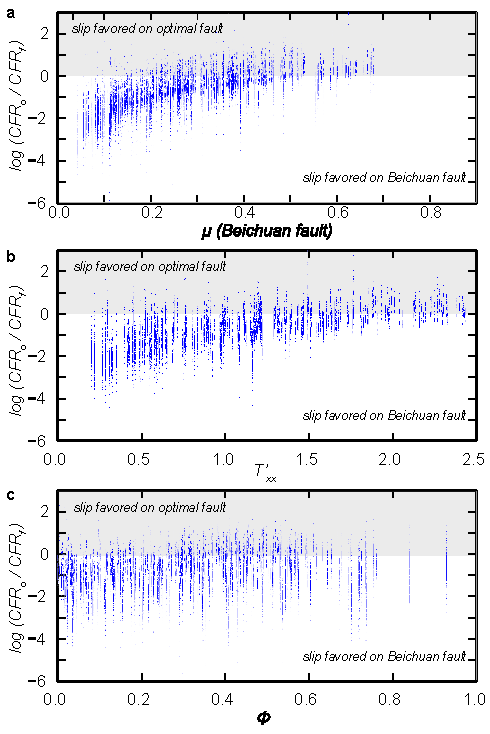
\includegraphics{../figures/cfr_plots.pdf}
\caption{Comparison of Coulomb failure ratio (CFR) on the Beichuan fault
from the \citet{zhang2011} coseismic slip model to CFR on an
optimally-oriented fault with $\mu = 0.6$, versus estimated $\mu$ on the
Beichuan fault. Values less than 0 (1 in linear space) indicate that
slip is favored on the Beichuan fault, even if it is not optimally
oriented. Values are calculated for each point in the slip model for
1000 randomly-drawn samples from $p(T,\mu,\phi |D)$.}
\label{fig:cfr_ratios}
\end{figure}

\begin{table}[htb]
\centering
\begin{tabular}{l c c c c}
\hline
Parameter & Coef. & Std. Err. & t statistic & $P>|t|$ \\
\hline
Intercept & -0.2566 & 0.0020 & -128.8 & \textless{}0.0001 \\ 
$\mu$ & 1.1168 & 0.0086 & 130.6 & \textless{}0.0001 \\ 
$T^\prime_{xx}$ & 0.9138 & 0.0048 & 191.2 & \textless{}0.0001 \\ 
$\phi$ & 0.5762 & 0.0055 & 105.7 & \textless{}0.0001 \\ 
\hline
\end{tabular}
\caption{Sensitivity of CFR ratios to relevant stress state parameters:
Results of multivariate linear regression of
$\mathrm{CFR}_o/ \mathrm{CFR}_f)$ against $\mu$, $\phi$ and
$T^\prime_{xx}$.}
\label{table:cfr_regress}
\end{table}

\subsection{The role of topography in orogenic development and strain
localization}\label{the-role-of-topography-in-orogenic-development-and-strain-localization}

Because the rise of broad elevated regions creates significant stresses
in the crust \citep[e.g.,][]{jeffreys1924}, these stresses have the
potential to influence orogenesis. The result may be to change the deformation
state in the interior of the orogen \citep[e.g.,][]{dewey1988, molnar1988}, the
convergence rates of the plates surrounding the orogen \citep[e.g.][]
{meade2008}, or the location and style of deformation at the orogen's
margins \citep[e.g.,][]{beaumont2001, decelles2009}. These studies show that
as an orogen rises, horizontal contraction via crustal thickening will
occur at the thin margins of the orogen, and if elevations reach a
threshold or tectonic compression decreases, extension will take place
in the orogen's high interior, as is well described in Tibet. Therefore,
Tibet is commonly suggested to be undergoing some manner of
gravitational collapse \citep[e.g.,][]{england1989}; where the plateau abuts
rigid cratons, the deformational patterns resemble `fixed boundary'
collapse \citep{rey2001}, with concentrated crustal thickening at the
orogen's margins \citep[e.g.,][]{cook2008}.

Though much work has been done exploring the feedback mechanisms between
topography and deformation; however, topography is typically greatly smoothed,
and topographic stresses are folded into gravitational potential energy
estimates of the entire lithosphere, and the whole lithospheric column
is often considered viscous \citep{copleymckenzie2007}. Therefore many
models seeking to predict deformation from gravitational forces yield
continuous deformation and do not consider how the gravitational
stresses resolve on heterogeneities embedded in the crust. However, the
presence of structures such as weak faults \citep{bird1994} or
low-viscosity channels or shear zones \citep[e.g.,][]{clark2005} can localize
deformation \citep[e.g.,][]{bird1994, fleschbendick2012}.

Our results that topographic stresses on the Wenchuan
earthquake faults are largely loaded in the opposite sense to the
coseismic slip direction indicates that gravitational collapse is probably
not the driver of reverse faulting in the Longmen Shan. However, as
noted previously, thrust flats in the middle crust present in some
coseismic slip models, particularly the Qi model, are loaded in a thrust
and dextral sense. Given the very low dips of the thrust flats
($0^{\circ}$--$5^{\circ}$), they receive very little loading from
horizontal tectonic stress, so any slip on them may be in response to
topographic loading and thus to gravitational collapse of the high
Longmen Shan and its hinterland. $M_{H{\mathrm{\max}}$ also changes
orientation from fault rangefront normal to closer to more oblique
near the front of the range (Figure \ref{fig:lms_topo_stresses_rot}),
suggesting that any transfer of mass from the highlands to the lowlands
due to topographic stresses should terminate near the rangefront.

However, because $M_{zz}$ is greater than $M_{H{\mathrm{max}}$
underneath the higher topography, topographic stresses can only lead to
reverse faulting on the Wenchuan faults if subhorizontal shear zones or
channels are present, and are very weak so shear can occur at 
low $\tau$ relative to $\sigma_n$. This conclusion has been reached in
studies of generalized orogens \citep[e.g.,][]{fleschbendick2012} and
gravitational collapse of volcanic edifices \citep[e.g.,][]{byrne2013},
indicating that is a general requirement of gravitational spreading. Our
calculations of $\mu$ and $\phi$ are based on $T$, which is biased
towards the high slip patches in the upper crust (Equation
\ref{eqn:rake_misfit}), yield low $\mu$ and low to moderate $\phi$,
which is probably insufficient for slip at high pressures at depth.
Similarly, a low viscosity horizontal
channel that underlies eastern Tibet, likely much deeper than the
seismogenic zone we consider here, would be able to flow in response to
$\tau$ regardless of $\sigma_n$ and may be able to facilitate
gravitational spreading of the orogen \citep[e.g.,][]{clark2005, cook2008,
fleschbendick2012}.

These arguments are all quite speculative, and we wish only to describe the
conditions under which gravitational collapse can occur given the
observations of deformation and the topographic stress field. It is not
at all clear that a suitably large decollement exists at the base of the
Beichuan fault (it is only present in one of the slip models
considered). Nonetheless, this topic has implications not only for
orogenic development, but for the recurrence interval on the Wenchuan
earthquake faults. If topographic stress contributes in some fashion to
the observed displacements on the fault, then those stresses were likely
barely diminished by coseismic stress change, and earthquake recurrence
of on the Wenchuan faults may be governed by different processes than
elastic rebound due to tectonic strain accumulation.

\section{Conclusions}\label{conclusions}

We have calculated shear and normal stresses due to topographic loading
on the Wenchuan earthquake faults, and used those stresses to constrain
tectonic stresses, fault friction and pore fluid pressure. Topographic
stresses on the main Wenchuan faults are large, with $\tau^M$ on the
faults up to \textbar{}20\textbar{} MPa, and $\sigma^M_n$ up to 80 MPa.
$\sigma^M_n$ reaches up to 100 MPa on mid-crustal thrust flats present
in some coseismic slip models. The direction of $\tau_M$ is generally
opposed to coseismic slip inferred during the 2008 Wenchuan earthquake,
indicating that weight of the topography resists coseismic slip. High
values of $\sigma^M_n$ increase the frictional resistance to slip,
potentially limiting slip magnitude in locations such as below the
Pengguan massif.

Assuming that the Beichuan faults were at a Mohr-Coulomb fault criterion
immediately prior to the Wenchuan earthquake, we estimate the tectonic
stresses required for the faults to fail. We use a Bayesian estimation,
resulting in posteriors representing likelihood of tectonic stress,
static friction, and a pore pressure parameter. The posteriors
indicate that the maximum tectonic stress is oriented
\textasciitilde{}E-W and has a likely minimum of 13.25 MPa km$^{-1}$.
The minimum tectonic stress is oriented \textasciitilde{}N-S and is
fairly low, with highest likelihood one half of the E-W tectonic stress.
The highest likelihood coefficient of static friction on the fault is
estimated at about 0.2--0.3, although values up to 0.5--0.6 are
permissable. Fluid pressures are likely 0--0.5 of the total pressure.

Slip occurred on these faults instead of more favorably-oriented faults
elsewhere in the region, due to the inferred low coefficient of friction
and moderate fluid pressures.

\appendix

\section{Green's functions for point-source
loads}\label{greens-functions-for-point-source-loads}
For completeness, we reproduce the Boussinesq \citep[e.g.,][]{jeffreys1970}
and Cerruti \citep[e.g.,][]{love1927} solutions here.
Note that in these solutions, $\lambda$ and $\mu$ are re-defined, and
are the first and second Lame's parameters, respectively, instead of
rake and fault friction as in the body of the manuscript.

\subsection{Boussinesq's solutions for vertical point-source
loads}\label{boussinesqs-solutions-for-vertical-point-source-loads}

\begin{equation}
\begin{split}
G_{xx}^B & = \frac{ F_v }{ 2\pi } \left[ \frac{ 3x^2 }{ r^5 } \right.
+ \frac{\mu (y^2 + z^2)}{(\lambda + \mu) r^3 (z + r)}
- \frac{\mu z}{(\lambda + \mu) r^3} \\
&\qquad \quad \left. - \frac{\mu x^2}{ (\lambda + \mu) r^2 (z + r)^2 }\right ]
\end{split}
\end{equation}

\begin{equation}
\begin{split}
G_{yy}^B & = \frac{F_v}{2\pi } \left [ \frac{3y^2}{r^5} \right.
+ \frac{\mu (x^{2} + z^{2})}{(\lambda + \mu) r^{3}(z + r)}
- \frac{\mu z}{(\lambda + \mu) r ^{3}} \\
& \qquad \quad \left. - \frac{\mu y^{2}}{(\lambda + \mu ) r^2 (z +r)^2} \right]
\end{split}
\end{equation}

\begin{equation}
G_{xy}^{B} = \frac{F _{v}}{2\pi} \left[ \frac{3xyz}{r^{5}}
- \frac{\mu x y (z + 2r)}{(\lambda + \mu) r^{3} (z + r)^{2}} \right]
\end{equation}

\begin{equation}
G_{zz}^{B} = 3 F _{v} z^{3} / 2 \pi r^{5}
\end{equation}

\begin{equation}
G_{xz}^{B} = 3 F _{v} xz^{2} / 2 \pi r^{5}
\end{equation}

\begin{equation}
G_{yz}^{B} = 3 F _{v} yz^{2} / 2 \pi r^{5}
\end{equation}

\subsection{Cerruti's solutions for horizontal point-source
loads}\label{cerrutis-solutions-for-horizontal-point-source-loads}

\begin{equation}
\begin{split}
G_{xx}^{C_x} &= \frac{ F_{h,x} x }{2 \pi r^3} \left[ \frac{ 3x^2}{r^2} \right.
- \frac{\mu}{(\lambda + \mu)(z+r)^2} 
\\
&\qquad \quad  \left. (r^2 - y^2 - \frac{2ry^2}{r+z}) \right]
\end{split}
\end{equation}

\begin{equation}
\begin{split}
G_{yy}^{C_x} & = \frac{ F_{h,x} x }{2 \pi r^3} \left[ \frac{ 3y^2}{r^2} \right.
- \frac{\mu}{(\lambda + \mu)(z+r)^2} \\
& \qquad \quad \left. (3r^2 - x^2 - \frac{2rx^2}{r+z}) \right]
\end{split}
\end{equation}

\begin{equation}
\begin{split}
G_{xy}^{C_x} & = \frac{ F_{h,x} x }{2 \pi r^3} \left[ \frac{ 3x^2}{r^2} \right.
- \frac{\mu}{(\lambda + \mu)(z+r)^2} 
\\
&\qquad \quad \left. \cdot (r^2 - x^2 - \frac{2rx^2}{r+z}) \right]
\end{split}
\end{equation}

\begin{equation}
    G^{C_x}_{zz} = \frac{ 3 F_{h,x} x z^2 }{2 \pi r^5}
\end{equation}

\begin{equation}
    G^{C_x}_{xz} = \frac{ 3 F_{h,x} z x^2 }{2 \pi r^5}
\end{equation}

\begin{equation}
    G^{C_x}_{yz} = \frac{ 3 F_{h,x} x y z }{2 \pi r^5}
\end{equation}

\begin{acknowledgements}
Joe Kington wrote the code to plot Figure \ref{fig:joint_posteriors}c.
\end{acknowledgements}
%\section{References}\label{references}

%\bibliography{wench_jgr_bib}{}
%\bibliographystyle{agufull08}

\begin{thebibliography}{87}
\providecommand{\natexlab}[1]{#1}
\expandafter\ifx\csname urlstyle\endcsname\relax
  \providecommand{\doi}[1]{doi:\discretionary{}{}{}#1}\else
  \providecommand{\doi}{doi:\discretionary{}{}{}\begingroup
  \urlstyle{rm}\Url}\fi

\bibitem[{\textit{Aagaard et~al.}(2001)\textit{Aagaard, Heaton, and
  Hall}}]{aagaard2001}
Aagaard, B.~T., T.~H. Heaton, and J.~F. Hall (2001), Dynamic earthquake
  ruptures in the presence of lithostatic normal stresses: {I}mplications for
  friction models and heat production, \textit{Bulletin of the Seismological
  Society of America}, \textit{91}(6), 1765--1796.

\bibitem[{\textit{Allmann and Shearer}(2009)}]{allmann2009}
Allmann, B.~P., and P.~M. Shearer (2009), Global variations of stress drop for
  moderate to large earthquakes, \textit{Journal of Geophysical Research: Solid
  Earth (1978--2012)}, \textit{114}(B1).

\bibitem[{\textit{Angelier}(1994)}]{angelier1994}
Angelier, J. (1994), Fault slip analysis and paleostress reconstruction,
  \textit{Continental deformation}, \textit{4}.

\bibitem[{\textit{Armijo et~al.}(1986)\textit{Armijo, Tapponnier, Mercier, and
  Han}}]{armijo1986}
Armijo, R., P.~Tapponnier, J.~Mercier, and T.-L. Han (1986), Quaternary
  extension in southern {T}ibet: {F}ield observations and tectonic
  implications, \textit{Journal of Geophysical Research: Solid Earth
  (1978--2012)}, \textit{91}(B14), 13,803--13,872.

\bibitem[{\textit{Beaumont et~al.}(2001)\textit{Beaumont, Jamieson, Nguyen, and
  Lee}}]{beaumont2001}
Beaumont, C., R.~A. Jamieson, M.~Nguyen, and B.~Lee (2001), Himalayan tectonics
  explained by extrusion of a low-viscosity crustal channel coupled to focused
  surface denudation, \textit{Nature}, \textit{414}(6865), 738--742.

\bibitem[{\textit{Bird and Kong}(1994)}]{bird1994}
Bird, P., and X.~Kong (1994), Computer simulations of {C}alifornia tectonics
  confirm very low strength of major faults, \textit{Geological Society of
  America Bulletin}, \textit{106}(2), 159--174.

\bibitem[{\textit{Bird and Piper}(1980)}]{birdpiper80}
Bird, P., and K.~Piper (1980), Plane-stress finite-element models of tectonic
  flow in southern {C}alifornia, \textit{Physics of the earth and planetary
  interiors}, \textit{21}(2), 158--175.

\bibitem[{\textit{Bollinger et~al.}(2004)\textit{Bollinger, Avouac, Cattin, and
  Pandey}}]{bollinger2004}
Bollinger, L., J.~Avouac, R.~Cattin, and M.~Pandey (2004), Stress buildup in
  the {H}imalaya, \textit{Journal of Geophysical Research: Solid Earth},
  \textit{109}(B11).

\bibitem[{\textit{Bott}(1959)}]{bott1959}
Bott, M. H.~P. (1959), The mechanics of oblique slip faulting,
  \textit{Geological Magazine}, \textit{96}(02), 109--117.

\bibitem[{\textit{Burchfiel et~al.}(1995)\textit{Burchfiel, Zhiliang, Yupinc,
  and Royden}}]{burchfiel1995}
Burchfiel, B., C.~Zhiliang, L.~Yupinc, and L.~Royden (1995), Tectonics of the
  {L}ongmen {S}han and adjacent regions, central {}china, \textit{International
  Geology Review}, \textit{37}(8), 661--735.

\bibitem[{\textit{Burchfiel et~al.}(2008)\textit{Burchfiel, Royden, van~der
  Hilst, Hager, Chen, King, Li, L{\"u}, Yao, and Kirby}}]{burchfiel2008}
Burchfiel, B., L.~Royden, R.~van~der Hilst, B.~Hager, Z.~Chen, R.~King, C.~Li,
  J.~L{\"u}, H.~Yao, and E.~Kirby (2008), A geological and geophysical context
  for the {W}enchuan earthquake of 12 {M}ay 2008, {S}ichuan, {P}eople's
  {R}epublic of {C}hina, \textit{GSA Today}, \textit{18}(7), 4--11.

\bibitem[{\textit{Byerlee}(1978)}]{byerlee1978}
Byerlee, J. (1978), Friction of rocks, \textit{Pure and applied Geophysics},
  \textit{116}(4-5), 615--626.

\bibitem[{\textit{Byrne et~al.}(2013)\textit{Byrne, Holohan, Kervyn, de~Vries,
  Troll, and Murray}}]{byrne2013}
Byrne, P., E.~Holohan, M.~Kervyn, B.~v.~W. de~Vries, V.~R. Troll, and J.~Murray
  (2013), A sagging-spreading continuum of large volcano structure,
  \textit{Geology}, \textit{41}(3), 339--342.

\bibitem[{\textit{Cattin et~al.}(1997)\textit{Cattin, Lyon-Caen, and
  Ch{\'e}ry}}]{cattin1997}
Cattin, R., H.~Lyon-Caen, and J.~Ch{\'e}ry (1997), Quantification of interplate
  coupling in subduction zones and forearc topography, \textit{Geophysical
  Research Letters}, \textit{24}(13), 1563--1566.

\bibitem[{\textit{Clark and Royden}(2000)}]{clarkroyden2000}
Clark, M.~K., and L.~H. Royden (2000), Topographic ooze: {B}uilding the eastern
  margin of {T}ibet by lower crustal flow, \textit{Geology}, \textit{28}(8),
  703--706.

\bibitem[{\textit{Clark et~al.}(2005)\textit{Clark, Bush, and
  Royden}}]{clark2005}
Clark, M.~K., J.~W. Bush, and L.~H. Royden (2005), Dynamic topography produced
  by lower crustal flow against rheological strength heterogeneities bordering
  the {T}ibetan {P}lateau, \textit{Geophysical Journal International},
  \textit{162}(2), 575--590.

\bibitem[{\textit{Coblentz and Richardson}(1996)}]{coblentz1996}
Coblentz, D.~D., and R.~M. Richardson (1996), Analysis of the {S}outh
  {A}merican intraplate stress field, \textit{Journal of Geophysical Research:
  Solid Earth (1978--2012)}, \textit{101}(B4), 8643--8657.

\bibitem[{\textit{Cook and Royden}(2008)}]{cook2008}
Cook, K.~L., and L.~H. Royden (2008), The role of crustal strength variations
  in shaping orogenic plateaus, with application to {T}ibet, \textit{Journal of
  Geophysical Research: Solid Earth (1978--2012)}, \textit{113}(B8).

\bibitem[{\textit{Copley and McKenzie}(2007)}]{copleymckenzie2007}
Copley, A., and D.~McKenzie (2007), Models of crustal flow in the
  {I}ndia--{A}sia collision zone, \textit{Geophysical Journal International},
  \textit{169}(2), 683--698.

\bibitem[{\textit{Copley et~al.}(2009)\textit{Copley, Boait, Hollingsworth,
  Jackson, and McKenzie}}]{copley2009}
Copley, A., F.~Boait, J.~Hollingsworth, J.~Jackson, and D.~McKenzie (2009),
  Subparallel thrust and normal faulting in {A}lbania and the roles of
  gravitational potential energy and rheology contrasts in mountain belts,
  \textit{Journal of Geophysical Research: Solid Earth}, \textit{114}(B5).

\bibitem[{\textit{Cui et~al.}(2014)\textit{Cui, Lin, Wang, Gao, Huang, Wang,
  Sun, Li, Zhou, Qian et~al.}}]{cui2014}
Cui, J., W.~Lin, L.~Wang, L.~Gao, Y.~Huang, W.~Wang, D.~Sun, Z.~Li, C.~Zhou,
  H.~Qian, et~al. (2014), Determination of three-dimensional in situ stresses
  by anelastic strain recovery in {W}enchuan {E}arthquake {F}ault {S}cientific
  {D}rilling {P}roject {H}ole-1 ({W}{F}{S}{D}-1), \textit{Tectonophysics},
  \textit{619–620}, 123 -- 132.

\bibitem[{\textit{Dahlen}(1990)}]{dahlen1990}
Dahlen, F. (1990), Critical taper model of fold-and-thrust belts and
  accretionary wedges, \textit{Annual Review of Earth and Planetary Sciences},
  \textit{18}, 55.

\bibitem[{\textit{Dalmayrac and Molnar}(1981)}]{dalmayrac1981}
Dalmayrac, B., and P.~Molnar (1981), Parallel thrust and normal faulting in
  {P}eru and constraints on the state of stress, \textit{Earth and Planetary
  Science Letters}, \textit{55}(3), 473--481.

\bibitem[{\textit{Day}(1982)}]{day1982}
Day, S.~M. (1982), Three-dimensional simulation of spontaneous rupture: {T}he
  effect of nonuniform prestress, \textit{Bulletin of the Seismological Society
  of America}, \textit{72}(6A), 1881--1902.

\bibitem[{\textit{DeCelles et~al.}(2009)\textit{DeCelles, Ducea, Kapp, and
  Zandt}}]{decelles2009}
DeCelles, P.~G., M.~N. Ducea, P.~Kapp, and G.~Zandt (2009), Cyclicity in
  cordilleran orogenic systems, \textit{Nature Geoscience}, \textit{2}(4),
  251--257.

\bibitem[{\textit{Dewey}(1988)}]{dewey1988}
Dewey, J.~F. (1988), Extensional collapse of orogens, \textit{Tectonics},
  \textit{7}(6), 1123--1139.

\bibitem[{\textit{England and Houseman}(1989)}]{england1989}
England, P., and G.~Houseman (1989), Extension during continental convergence,
  with application to the tibetan plateau, \textit{Journal of Geophysical
  Research: Solid Earth (1978--2012)}, \textit{94}(B12), 17,561--17,579.

\bibitem[{\textit{Farr et~al.}(2007)\textit{Farr, Rosen, Caro, Crippen, Duren,
  Hensley, Kobrick, Paller, Rodriguez, Roth et~al.}}]{farr2007srtm}
Farr, T.~G., P.~A. Rosen, E.~Caro, R.~Crippen, R.~Duren, S.~Hensley,
  M.~Kobrick, M.~Paller, E.~Rodriguez, L.~Roth, et~al. (2007), The shuttle
  radar topography mission, \textit{Reviews of geophysics}, \textit{45}(2).

\bibitem[{\textit{Feng et~al.}(2010)\textit{Feng, Hetland, Ding, Li, and
  Zhang}}]{feng2010}
Feng, G., E.~A. Hetland, X.~Ding, Z.~Li, and L.~Zhang (2010), Coseismic fault
  slip of the 2008 {M}w 7.9 {W}enchuan earthquake estimated from {I}n{S}{A}{R}
  and {G}{P}{S} measurements, \textit{Geophysical research letters},
  \textit{37}(1).

\bibitem[{\textit{Fielding et~al.}(2013)\textit{Fielding, Sladen, Li, Avouac,
  B{\"u}rgmann, and Ryder}}]{fielding2013}
Fielding, E.~J., A.~Sladen, Z.~Li, J.-P. Avouac, R.~B{\"u}rgmann, and I.~Ryder
  (2013), Kinematic fault slip evolution source models of the 2008 m7.9
  wenchuan earthquake in china from sar interferometry, gps and teleseismic
  analysis and implications for longmen shan tectonics, \textit{Geophysical
  Journal International}, \textit{194}(2), 1138--1166.

\bibitem[{\textit{Flesch and Bendick}(2012)}]{fleschbendick2012}
Flesch, L., and R.~Bendick (2012), The relationship between surface kinematics
  and deformation of the whole lithosphere, \textit{Geology}, \textit{40}(8),
  711--714.

\bibitem[{\textit{Flesch and Kreemer}(2010)}]{flesch2010gpe}
Flesch, L.~M., and C.~Kreemer (2010), Gravitational potential energy and
  regional stress and strain rate fields for continental plateaus: {E}xamples
  from the central {A}ndes and {C}olorado {P}lateau, \textit{Tectonophysics},
  \textit{482}(1), 182--192.

\bibitem[{\textit{Heidbach et~al.}(2009)\textit{Heidbach, Tingay, and
  Barth}}]{heidbach2009}
Heidbach, O., M.~Tingay, and A.~Barth (2009), \textit{The World Stress Map
  based on the database release 2008, equatorial scale 1:46,000,000},
  Commission for the Geological Map of the World, Paris.

\bibitem[{\textit{Hubbard et~al.}(2010)\textit{Hubbard, Shaw, and
  Klinger}}]{hubbard2010}
Hubbard, J., J.~H. Shaw, and Y.~Klinger (2010), Structural setting of the 2008
  {M}w 7.9 {W}enchuan, {C}hina, earthquake, \textit{Bulletin of the
  Seismological Society of America}, \textit{100}(5B), 2713--2735.

\bibitem[{\textit{Jarvis et~al.}(2008)\textit{Jarvis, Reuter, Nelson, and
  Guevara}}]{jarvis2008srtm}
Jarvis, A., H.~Reuter, A.~Nelson, and E.~Guevara (2008), Hole-filled srtm for
  the globe version 3, available from the cgiar-csi srtm 90m database,
  \textit{Accessed: March}, \textit{12}, 2012.

\bibitem[{\textit{Jeffreys}(1924)}]{jeffreys1924}
Jeffreys, H. (1924), \textit{The Earth: its origin, history and physical
  constitution}, Cambridge University Press.

\bibitem[{\textit{Jeffreys}(1970)}]{jeffreys1970}
Jeffreys, H. (1970), \textit{The Earth}, Cambridge University Press.

\bibitem[{\textit{Kanamori and Anderson}(1975)}]{kanamori1975}
Kanamori, H., and D.~L. Anderson (1975), Theoretical basis of some empirical
  relations in seismology, \textit{Bulletin of the Seismological Society of
  America}, \textit{65}(5), 1073--1095.

\bibitem[{\textit{Kuo et~al.}(2014)\textit{Kuo, Li, Smith, Di~Toro, Suppe,
  Song, Nielsen, Sheu, and Si}}]{kuo2014}
Kuo, L.-W., H.~Li, S.~A. Smith, G.~Di~Toro, J.~Suppe, S.-R. Song, S.~Nielsen,
  H.-S. Sheu, and J.~Si (2014), Gouge graphitization and dynamic fault
  weakening during the 2008 {M}w 7.9 {W}enchuan earthquake, \textit{Geology},
  \textit{42}(1), 47--50.

\bibitem[{\textit{Lamb}(2006)}]{lamb2006}
Lamb, S. (2006), Shear stresses on megathrusts: {I}mplications for mountain
  building behind subduction zones, \textit{Journal of Geophysical Research:
  Solid Earth}, \textit{111}(B7).

\bibitem[{\textit{Liang et~al.}(2013)\textit{Liang, Gan, Shen, Xiao, Liu, Chen,
  Ding, and Zhou}}]{liang2013}
Liang, S., W.~Gan, C.~Shen, G.~Xiao, J.~Liu, W.~Chen, X.~Ding, and D.~Zhou
  (2013), Three-dimensional velocity field of present-day crustal motion of the
  {T}ibetan {P}lateau derived from {G}{P}{S} measurements, \textit{Journal of
  Geophysical Research: Solid Earth}, \textit{118}(10), 5722--5732.

\bibitem[{\textit{Lin et~al.}(2009)\textit{Lin, Ren, Jia, and Wu}}]{lin2009}
Lin, A., Z.~Ren, D.~Jia, and X.~Wu (2009), Co-seismic thrusting rupture and
  slip distribution produced by the 2008< i> m</i>< sub> w</sub> 7.9 {W}enchuan
  earthquake, china, \textit{Tectonophysics}, \textit{471}(3), 203--215.

\bibitem[{\textit{Lisle}(2013)}]{lisle2013}
Lisle, R.~J. (2013), A critical look at the {W}allace-{B}ott hypothesis in
  fault-slip analysis, \textit{Bulletin de la Societe Geologique de France},
  \textit{184}(4-5), 299--306.

\bibitem[{\textit{Liu and Zoback}(1992)}]{liuzoback1992}
Liu, L., and M.~D. Zoback (1992), The effect of topography on the state of
  stress in the crust: {A}pplication to the site of the {C}ajon {P}ass
  {S}cientific {D}rilling {P}roject, \textit{Journal of Geophysical Research:
  Solid Earth (1978--2012)}, \textit{97}(B4), 5095--5108.

\bibitem[{\textit{Liu and Yang}(2003)}]{liuyang2003}
Liu, M., and Y.~Yang (2003), Extensional collapse of the {T}ibetan {P}lateau:
  {R}esults of three-dimensional finite element modeling, \textit{Journal of
  Geophysical Research: Solid Earth (1978--2012)}, \textit{108}(B8).

\bibitem[{\textit{Liu-Zeng et~al.}(2009)\textit{Liu-Zeng, Zhang, Wen,
  Tapponnier, Sun, Xing, Hu, Xu, Zeng, Ding et~al.}}]{liu2009}
Liu-Zeng, J., Z.~Zhang, L.~Wen, P.~Tapponnier, J.~Sun, X.~Xing, G.~Hu, Q.~Xu,
  L.~Zeng, L.~Ding, et~al. (2009), Co-seismic ruptures of the 12 may 2008,< i>
  m</i>< sub> s</sub> 8.0 wenchuan earthquake, sichuan: East--west crustal
  shortening on oblique, parallel thrusts along the eastern edge of tibet,
  \textit{Earth and Planetary Science Letters}, \textit{286}(3), 355--370.

\bibitem[{\textit{Love}(1927)}]{love1927}
Love, E.~A.~H. (1927), \textit{The mathematical theory of elasticity.},
  Cambridge University Press.

\bibitem[{\textit{Loveless and Meade}(2011)}]{loveless2011}
Loveless, J., and B.~Meade (2011), Partitioning of localized and diffuse
  deformation in the {T}ibetan {P}lateau from joint inversions of geologic and
  geodetic observations, \textit{Earth and Planetary Science Letters},
  \textit{303}(1), 11--24.

\bibitem[{\textit{Luttrell et~al.}(2007)\textit{Luttrell, Sandwell,
  Smith-Konter, Bills, and Bock}}]{luttrell2007}
Luttrell, K., D.~Sandwell, B.~Smith-Konter, B.~Bills, and Y.~Bock (2007),
  Modulation of the earthquake cycle at the southern {S}an {A}ndreas fault by
  lake loading, \textit{Journal of Geophysical Research: Solid Earth
  (1978--2012)}, \textit{112}(B8).

\bibitem[{\textit{Luttrell et~al.}(2011)\textit{Luttrell, Tong, Sandwell,
  Brooks, and Bevis}}]{luttrell2011}
Luttrell, K.~M., X.~Tong, D.~T. Sandwell, B.~A. Brooks, and M.~G. Bevis (2011),
  Estimates of stress drop and crustal tectonic stress from the 27 {F}ebruary
  2010 {M}aule, {C}hile, earthquake: Implications for fault strength,
  \textit{Journal of Geophysical Research: Solid Earth}, \textit{116}(B11).

\bibitem[{\textit{Martel}(2006)}]{martel2006}
Martel, S.~J. (2006), Effect of topographic curvature on near-surface stresses
  and application to sheeting joints, \textit{Geophysical Research Letters},
  \textit{33}(1).

\bibitem[{\textit{McKenzie}(1969)}]{mckenzie1969}
McKenzie, D.~P. (1969), The relation between fault plane solutions for
  earthquakes and the directions of the principal stresses, \textit{Bulletin of
  the Seismological Society of America}, \textit{59}(2), 591--601.

\bibitem[{\textit{McKinney}(2010)}]{mckinney2010}
McKinney, W. (2010), Data structures for statistical computing in python, in
  \textit{Proceedings of the 9th Python in Science Conference}, edited by
  S.~van~der Walt and J.~Millman, pp. 51 -- 56, SciPy.

\bibitem[{\textit{McTigue and Mei}(1981)}]{mctiguemei1981}
McTigue, D.~F., and C.~C. Mei (1981), Gravity-induced stresses near topography
  of small slope, \textit{Journal of Geophysical Research: Solid Earth},
  \textit{86}(B10), 9268--9278.

\bibitem[{\textit{Meade and Conrad}(2008)}]{meade2008}
Meade, B.~J., and C.~P. Conrad (2008), Andean growth and the deceleration of
  {S}outh {A}merican subduction: {T}ime evolution of a coupled
  orogen-subduction system, \textit{Earth and Planetary Science Letters},
  \textit{275}(1), 93--101.

\bibitem[{\textit{Medina~Luna and Hetland}(2013)}]{medinaluna2013}
Medina~Luna, L., and E.~A. Hetland (2013), Regional stresses inferred from
  coseismic slip models of the 2008 {M}w 7.9 {W}enchuan, {C}hina, earthquake,
  \textit{Tectonophysics}, \textit{584}, 43--53.

\bibitem[{\textit{Meissner and Strehlau}(1982)}]{meissner1982}
Meissner, R., and J.~Strehlau (1982), Limits of stresses in continental crusts
  and their relation to the depth-frequency distribution of shallow
  earthquakes, \textit{Tectonics}, \textit{1}(1), 73--89.

\bibitem[{\textit{Michael}(1987)}]{michael1987}
Michael, A.~J. (1987), Use of focal mechanisms to determine stress: a control
  study, \textit{Journal of Geophysical Research: Solid Earth (1978--2012)},
  \textit{92}(B1), 357--368.

\bibitem[{\textit{Miller and Dunne}(1996)}]{millerdunne1996}
Miller, D.~J., and T.~Dunne (1996), Topographic perturbations of regional
  stresses and consequent bedrock fracturing, \textit{Journal of Geophysical
  Research: Solid Earth (1978--2012)}, \textit{101}(B11), 25,523--25,536.

\bibitem[{\textit{Molnar and Lyon-Caen}(1988)}]{molnar1988}
Molnar, P., and H.~Lyon-Caen (1988), Some simple physical aspects of the
  support, structure, and evolution of mountain belts, \textit{Spec. Pap. Geol.
  Soc. Am}, \textit{218}, 179--207.

\bibitem[{\textit{Mosegaard and Tarantola}(1995)}]{mosegaard1995}
Mosegaard, K., and A.~Tarantola (1995), Monte {C}arlo sampling of solutions to
  inverse problems, \textit{Journal of Geophysical Research: Solid Earth
  (1978--2012)}, \textit{100}(B7), 12,431--12,447.

\bibitem[{\textit{Nakamura et~al.}(2010)\textit{Nakamura, Tsuboi, Kaneda, and
  Yamanaka}}]{nakamura2010}
Nakamura, T., S.~Tsuboi, Y.~Kaneda, and Y.~Yamanaka (2010), Rupture process of
  the 2008 {W}enchuan, {C}hina earthquake inferred from teleseismic waveform
  inversion and forward modeling of broadband seismic waves,
  \textit{Tectonophysics}, \textit{491}(1), 72--84.

\bibitem[{\textit{Oglesby and Day}(2002)}]{oglesbyday2002}
Oglesby, D.~D., and S.~M. Day (2002), Stochastic fault stress: {I}mplications
  for fault dynamics and ground motion, \textit{Bulletin of the Seismological
  Society of America}, \textit{92}(8), 3006--3021.

\bibitem[{\textit{Oliphant}(2007)}]{oliphant2007numpy}
Oliphant, T.~E. (2007), Python for scientific computing, \textit{Computing in
  Science \& Engineering}, \textit{9}(3), 10--20.

\bibitem[{\textit{Olsen et~al.}(1997)\textit{Olsen, Madariaga, and
  Archuleta}}]{olsen1997}
Olsen, K., R.~Madariaga, and R.~Archuleta (1997), Three-dimensional dynamic
  simulation of the 1992 {L}anders earthquake, \textit{Science},
  \textit{278}(5339), 834--838.

\bibitem[{\textit{P\'erez and Granger}(2007)}]{perez2007ipython}
P\'erez, F., and B.~E. Granger (2007), {IP}ython: a {S}ystem for {I}nteractive
  {S}cientific {C}omputing, \textit{{C}omput. {S}ci. {E}ng.}, \textit{9}(3),
  21--29.

\bibitem[{\textit{Qi et~al.}(2011)\textit{Qi, Xuejun, Qigui, Freymueller,
  Shaomin, Caijun, Yonglin, Xinzhao, Kai, and Gang}}]{qi2011}
Qi, W., Q.~Xuejun, L.~Qigui, J.~Freymueller, Y.~Shaomin, X.~Caijun, Y.~Yonglin,
  Y.~Xinzhao, T.~Kai, and C.~Gang (2011), Rupture of deep faults in the 2008
  {W}enchuan earthquake and uplift of the {L}ongmen {S}han, \textit{Nature
  Geoscience}, \textit{4}(9), 634--640.

\bibitem[{\textit{Reches}(1987)}]{reches1987}
Reches, Z. (1987), Determination of the tectonic stress tensor from slip along
  faults that obey the coulomb yield condition, \textit{Tectonics},
  \textit{6}(6), 849--861.

\bibitem[{\textit{Rey et~al.}(2001)\textit{Rey, Vanderhaeghe, and
  Teyssier}}]{rey2001}
Rey, P., O.~Vanderhaeghe, and C.~Teyssier (2001), Gravitational collapse of the
  continental crust: definition, regimes and modes, \textit{Tectonophysics},
  \textit{342}(3), 435--449.

\bibitem[{\textit{Richardson and Coblentz}(1994)}]{richardson1994}
Richardson, R.~M., and D.~D. Coblentz (1994), Stress modeling in the {A}ndes:
  Constraints on the {S}outh {A}merican intraplate stress magnitudes,
  \textit{Journal of Geophysical Research: Solid Earth}, \textit{99}(B11),
  22,015--22,025.

\bibitem[{\textit{Savage and Swolfs}(1986)}]{savageswolfs1986}
Savage, W.~Z., and H.~S. Swolfs (1986), Tectonic and gravitational stress in
  long symmetric ridges and valleys, \textit{Journal of Geophysical Research:
  Solid Earth}, \textit{91}(B3), 3677--3685.

\bibitem[{\textit{Scholz}(2002)}]{scholz2002}
Scholz, C.~H. (2002), \textit{The mechanics of earthquakes and faulting},
  Cambridge university press.

\bibitem[{\textit{Seabold and Perktold}(2010)}]{seabold2010}
Seabold, S., and J.~Perktold (2010), Statsmodels: econometric and statistical
  modeling with python, in \textit{Proceedings of the 9th Python in Science
  Conference}, pp. 57--61, SciPy.

\bibitem[{\textit{Shen et~al.}(2009)\textit{Shen, Sun, Zhang, Wan, Wang,
  B{\"u}rgmann, Zeng, Gan, Liao, and Wang}}]{shen2009}
Shen, Z.-K., J.~Sun, P.~Zhang, Y.~Wan, M.~Wang, R.~B{\"u}rgmann, Y.~Zeng,
  W.~Gan, H.~Liao, and Q.~Wang (2009), Slip maxima at fault junctions and
  rupturing of barriers during the 2008 {W}enchuan earthquake, \textit{Nature
  Geoscience}, \textit{2}(10), 718--724.

\bibitem[{\textit{Sibson}(1985)}]{sibson1985}
Sibson, R.~H. (1985), A note on fault reactivation, \textit{Journal of
  Structural Geology}, \textit{7}(6), 751--754.

\bibitem[{\textit{Styron et~al.}(2010)\textit{Styron, Taylor, and
  Okoronkwo}}]{styron2010}
Styron, R., M.~Taylor, and K.~Okoronkwo (2010), Database of active structures
  from the {I}ndo-{A}sian collision, \textit{Eos, Transactions American
  Geophysical Union}, \textit{91}(20), 181--182.

\bibitem[{\textit{Tarantola}(2005)}]{tarantola2005}
Tarantola, A. (2005), \textit{Inverse problem theory and methods for model
  parameter estimation}, SIAM.

\bibitem[{\textit{Taylor et~al.}(2003)\textit{Taylor, Yin, Ryerson, Kapp, and
  Ding}}]{taylor2003}
Taylor, M., A.~Yin, F.~J. Ryerson, P.~Kapp, and L.~Ding (2003), Conjugate
  strike-slip faulting along the {B}angong-{N}ujiang suture zone accommodates
  coeval east-west extension and north-south shortening in the interior of the
  {T}ibetan {P}lateau, \textit{Tectonics}, \textit{22}(4).

\bibitem[{\textit{Tong et~al.}(2010)\textit{Tong, Sandwell, and
  Fialko}}]{tong2010}
Tong, X., D.~T. Sandwell, and Y.~Fialko (2010), Coseismic slip model of the
  2008 {W}enchuan earthquake derived from joint inversion of interferometric
  synthetic aperture radar, {G}{P}{S}, and field data, \textit{Journal of
  Geophysical Research: Solid Earth}, \textit{115}(B4).

\bibitem[{\textit{Townend and Zoback}(2000)}]{townend2000}
Townend, J., and M.~D. Zoback (2000), How faulting keeps the crust strong,
  \textit{Geology}, \textit{28}(5), 399--402.

\bibitem[{\textit{Wallace}(1951)}]{wallace1951}
Wallace, R.~E. (1951), Geometry of shearing stress and relation to faulting,
  \textit{The Journal of Geology}, pp. 118--130.

\bibitem[{\textit{Wang et~al.}(2012)\textit{Wang, Kirby, Furlong, Van~Soest,
  Xu, Shi, Kamp, and Hodges}}]{wang2012}
Wang, E., E.~Kirby, K.~P. Furlong, M.~Van~Soest, G.~Xu, X.~Shi, P.~J. Kamp, and
  K.~Hodges (2012), Two-phase growth of high topography in eastern {T}ibet
  during the {C}enozoic, \textit{Nature Geoscience}, \textit{5}(9), 640--645.

\bibitem[{\textit{Xiao et~al.}(1991)\textit{Xiao, Dahlen, and
  Suppe}}]{xiao1991}
Xiao, H.-B., F.~Dahlen, and J.~Suppe (1991), Mechanics of extensional wedges,
  \textit{Journal of Geophysical Research: Solid Earth}, \textit{96}(B6),
  10,301--10,318.

\bibitem[{\textit{Xu et~al.}(2009)\textit{Xu, Wen, Yu, Chen, Klinger, Hubbard,
  and Shaw}}]{xu2009}
Xu, X., X.~Wen, G.~Yu, G.~Chen, Y.~Klinger, J.~Hubbard, and J.~Shaw (2009),
  Coseismic reverse-and oblique-slip surface faulting generated by the 2008 mw
  7.9 wenchuan earthquake, china, \textit{Geology}, \textit{37}(6), 515--518.

\bibitem[{\textit{Yong et~al.}(2003)\textit{Yong, Allen, Densmore, and
  Qiang}}]{yong2003}
Yong, L., P.~A. Allen, A.~L. Densmore, and X.~Qiang (2003), Evolution of the
  {L}ongmen {S}han foreland basin (western {S}ichuan, {C}hina) during the
  {L}ate {T}riassic {I}ndosinian orogeny, \textit{Basin Research},
  \textit{15}(1), 117--138.

\bibitem[{\textit{Zhang et~al.}(2011)\textit{Zhang, Qu, Shan, Song, Zhang,
  Wang, Hu, and Wang}}]{zhang2011}
Zhang, G., C.~Qu, X.~Shan, X.~Song, G.~Zhang, C.~Wang, J.-C. Hu, and R.~Wang
  (2011), Slip distribution of the 2008 {W}enchuan {M}s 7.9 earthquake by joint
  inversion from {G}{P}{S} and {I}n{S}{A}{R} measurements: a resolution test
  study, \textit{Geophysical Journal International}, \textit{186}(1), 207--220.

\bibitem[{\textit{Zhang et~al.}(2010)\textit{Zhang, Wen, Shen, and
  Chen}}]{zhang2010}
Zhang, P.-Z., X.-z. Wen, Z.-K. Shen, and J.-h. Chen (2010), Oblique,
  high-angle, listric-reverse faulting and associated development of strain:
  The {W}enchuan earthquake of {M}ay 12, 2008, {S}ichuan, {C}hina,
  \textit{Annual Review of Earth and Planetary Sciences}, \textit{38},
  353--382.

\end{thebibliography}


\end{article}

\end{document}
